%!TEX root = ../main.tex
\chapter{Campi elettrici e magnetici lentamente variabili}

Il ritardo di propagazione è breve perché la velocità della luce è altissima. Il fenomeno è lentamente variabile se la scala temporale su cui si presenta la corrente è molto più lunga del ritardo temporale di propagazione dell'informazione. In regime lentamente variabile facciamo finta che $\vec{B}$ giunga istantaneamente nel punto in cui stiamo calcolando il campo.

\[
	\vec{B} (P)=\vec{B} (t-\tau) \simeq \vec{B} (t)=\frac{\mu_0 I(t)}{2\pi d}\vec{u}_{\varphi}
\]

I ritardi diventano essenziali quando si affronta la propagazione di onde elettromagnetiche.
Le proprietà locali dei campi elettrici e magnetici costanti nel tempo sono stabilite nel vuoto dalle quattro equazioni di Maxwell studiate. La condizione di stazionarietà è evidenziata dal fatto che nelle equazioni compaiono solo le derivate rispetto alle coordinate spaziali e non quelle rispetto al tempo. A parte il fatto che il campo magnetico statico $\vec{B}$ è generato da cariche elettriche in movimento, non esiste in un dato sistema di riferimento inerziale nessun'altra connessione tra i fenomeni elettrici e magnetici statici e le relative coppie di equazioni possono essere risolte separatamente. Esperimenti condotti da Faraday e da Henry separatamente misero in evidenza una diversa connessione tra elettricità e magnetismo: un campo magnetico variabile nel tempo genera un campo elettrico non conservativo che in opportuni dispositivi può dar luogo a una forza elettromotrice e ad una corrente in un circuito chiuso. Maxwell arrivò poi a una forma più generale delle equazioni che regolano i fenomeni elettrici e magnetici visibili, che contengono le quattro equazioni già studiate per il caso stazionario come caso limite. Caratteristica fondamentale è che un campo elettrico e un campo magnetico variabili non possono esistere separatamente, ma vanno riuniti sotto il concetto più generale di campo elettromagnetico.

\section{Induzione elettromagnetica}

Dal momento che abbiamo studiato il fenomeno dell'induzione elettrostatica, potremmo chiederci se esiste un fenomeno analogo anche nel caso del magnetismo.
Se si avvicina un magnete ad una spira $A$ connessa con un galvanometro, il suo indice si sposta in una certa direzione, se lo si allontana, la direzione dello spostamento sarà quella opposta. Quando il magnete è fermo rispetto alla spira non si osserva nessuno spostamento dell'indice dello strumento. Già da questo fatto si intuisce che in una situazione in quiete non può essere indotta una corrente su un filo. Gli effetti sono uguali se si tiene fermo il magnete e si avvicina o si allontana la spira. Se sostituiamo il magnete con una spira $\vec{B}$ in cui è inserito un generatore che fa circolare corrente e muoviamo $\vec{B}$ rispetto ad $A$ o $A$ rispetto a $\vec{B}$, si ottiene lo stesso effetto. Da tali osservazioni si può concludere che in una spira compare una corrente, che chiamiamo indotta, ogni qual volta c'è un moto relativo tra la spira e un campo magnetico $\vec{B}$, generato da un magnete permanente o da un'altra spira percorsa da corrente.
Dall'esame quantitativo dei casi descritti e di tutte le altre situazioni in cui si manifesta il fenomeno dell'induzione, Faraday dedusse che \emph{ogni qual volta il flusso del campo magnetico $\Phi (\vec{B})$ concatenato con un circuito varia nel tempo, si ha nel circuito una forza elettromotrice indotta data dall'opposto della derivata del flusso rispetto al tempo}:

\[
	\boxed{f_i = - \frac{d\Phi_{\Sigma}(\vec{B} )}{dt}}
\]

Tale risultato è detto \textbf{legge di Faraday-Neumann}.
La forza elettromotrice è definita come integrale del campo elettrico $\vec{E}$ lungo una linea chiusa, cioè come la circuitazione di $ \vec{E}  $

\[
	f_i=\oint_{\gamma} \vec{E}_e  \cdot d\vec{l} \neq 0
\]

e un suo valore non nullo implica che il campo elettrico non è conservativo.

\begin{figure}[htpb]
	\centering

	\tikzset{every picture/.style={line width=0.75pt}} %set default line width to 0.75pt        

	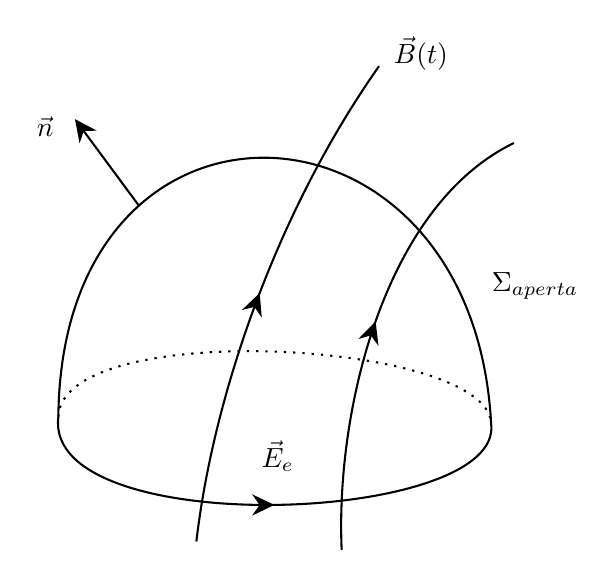
\begin{tikzpicture}[x=0.75pt,y=0.75pt,yscale=-1,xscale=1]
	%uncomment if require: \path (0,300); %set diagram left start at 0, and has height of 300

	%Curve Lines [id:da9896045425165532] 
	\draw    (210,211) .. controls (202.5,271) and (425.5,263) .. (418.5,214) ;
	\draw [shift={(314.06,253.38)}, rotate = 539.9200000000001] [fill={rgb, 255:red, 0; green, 0; blue, 0 }  ][line width=0.08]  [draw opacity=0] (10.72,-5.15) -- (0,0) -- (10.72,5.15) -- (7.12,0) -- cycle    ;
	%Curve Lines [id:da47209199424878445] 
	\draw  [dash pattern={on 0.84pt off 2.51pt}]  (210,211) .. controls (211.5,163) and (416.5,174) .. (418.5,214) ;
	%Curve Lines [id:da13680608874761813] 
	\draw    (210,211) .. controls (211.5,40) and (409.5,48) .. (418.5,214) ;
	%Straight Lines [id:da8930151161079218] 
	\draw    (248.67,109) -- (219.78,69.91) ;
	\draw [shift={(218,67.5)}, rotate = 413.53999999999996] [fill={rgb, 255:red, 0; green, 0; blue, 0 }  ][line width=0.08]  [draw opacity=0] (10.72,-5.15) -- (0,0) -- (10.72,5.15) -- (7.12,0) -- cycle    ;
	%Curve Lines [id:da39004395489350374] 
	\draw    (346.5,275) .. controls (343.5,207) and (367.5,109) .. (429.5,79) ;
	\draw [shift={(362.83,164.96)}, rotate = 468.8] [fill={rgb, 255:red, 0; green, 0; blue, 0 }  ][line width=0.08]  [draw opacity=0] (10.72,-5.15) -- (0,0) -- (10.72,5.15) -- (7.12,0) -- cycle    ;
	%Curve Lines [id:da616401806299091] 
	\draw    (276.5,271) .. controls (284.5,202) and (314.5,113) .. (364.5,42) ;
	\draw [shift={(307,151.29)}, rotate = 470.75] [fill={rgb, 255:red, 0; green, 0; blue, 0 }  ][line width=0.08]  [draw opacity=0] (10.72,-5.15) -- (0,0) -- (10.72,5.15) -- (7.12,0) -- cycle    ;

	% Text Node
	\draw (439.67,148) node    {$\Sigma _{\text{aperta}}$};
	% Text Node
	\draw (203.67,71) node    {$\vec{n}$};
	% Text Node
	\draw (384.67,36) node    {$\vec{B}( t)$};
	% Text Node
	\draw (315.67,230) node    {$\vec{E}_{e}$};

	\end{tikzpicture}
\end{figure}
\FloatBarrier

\emph{Esempio.}
Immaginiamo di considerare un circuito $ \gamma  $ a cui diamo un verso arbitrario di percorrenza. Individuiamo una superficie $\Sigma$ aperta che abbia $\gamma$ come orlo. Associamo con la regola del cavatappi a $\Sigma$ una normale. Supponiamo che in questa regione dello spazio sia presente un campo magnetico variabile nel tempo. Chiamiamo il flusso concatenato al circuito flusso di $\vec{B}$ attraverso la superficie $\Sigma$ (non dipende dalla superficie). Se la variazione di campo magnetico produce una forza elettromotrice nel circuito, possiamo immaginare che vi sia un campo elettromotore $\vec{E}_e $. Possiamo calcolare la \textbf{forza elettromotrice indotta}:

\[
	f_i = - \frac{d\Phi_{\Sigma}(\vec{B} )}{dt}
\]

La legge afferma che tale $fem$ è pari all'opposto derivata rispetto al tempo del flusso concatenato al circuito.
Tutte le casistiche viste separatamente si riuniscono sotto quest'unica legge. Il segno meno può essere interpretato in forma pratica. La forza elettromotrice si oppone alla causa che la sta generando. La corrente gira in modo da generare un campo magnetico che si oppone all'aumento di flusso. Viceversa se $\vec{B}$ sta diminuendo (e quindi anche il flusso) la corrente indotta cerca di rafforzare il flusso. Questo particolare enunciato è noto come \textbf{legge di Lenz}.

Esaminiamo ora come si realizza una variazione di flusso nel tempo, elencando prima le varie possibilità:

\begin{itemize}
	\item si ha sempre una variazione del flusso quando un circuito indeformabile si muove (trasla, ruota) in un campo magnetico. L'unica eccezione è il caso di moto traslatorio in un campo uniforme.
	\item Deformazione del circuito. Si ha il moto di una sua singola parte o anche soltanto di qualche parte. Il flusso concatenato con il circuito in generale cambia nel tempo. Il fenomeno avviene sia con un campo uniforme che con un campo non uniforme.
	\item Si mantiene il circuito fisso e si sposta la sorgente con del campo magnetico.
	\item Con circuito fisso e sorgenti di $\vec{B}$ fisse il flusso concatenato cambia nel tempo se si muove un mezzo ferromagnetico magnetizzato.
	\item In assenza di qualsiasi moto relativo tra circuito e campo magnetico e di variazioni locali di permeabilità magnetica, si ha una variazione di flusso attraverso il circuito se il campo magnetico, uniforme o no, varia nel tempo a causa della variazione nel tempo dell'intensità della corrente che lo genera.
\end{itemize}

Supponiamo che ci sia una sorgente di campo magnetico non uniforme. Poniamo che in tale regione dello spazio sia presente un circuito a cui diamo un verso di percorrenza e una normale alla superficie $\Sigma$ avente $\gamma$ come contorno. Il circuito in quiete viene spostato di moto di pura traslazione nella regione in cui è presente campo magnetico con velocità $\vec{v}$. Consideriamo una delle varie cariche presenti nel circuito.

\begin{figure}[htpb]
	\centering

	% Pattern Info
	 
	\tikzset{
	pattern size/.store in=\mcSize, 
	pattern size = 5pt,
	pattern thickness/.store in=\mcThickness, 
	pattern thickness = 0.3pt,
	pattern radius/.store in=\mcRadius, 
	pattern radius = 1pt}
	\makeatletter
	\pgfutil@ifundefined{pgf@pattern@name@_rlc9ed9hs}{
	\pgfdeclarepatternformonly[\mcThickness,\mcSize]{_rlc9ed9hs}
	{\pgfqpoint{0pt}{0pt}}
	{\pgfpoint{\mcSize+\mcThickness}{\mcSize+\mcThickness}}
	{\pgfpoint{\mcSize}{\mcSize}}
	{
	\pgfsetcolor{\tikz@pattern@color}
	\pgfsetlinewidth{\mcThickness}
	\pgfpathmoveto{\pgfqpoint{0pt}{0pt}}
	\pgfpathlineto{\pgfpoint{\mcSize+\mcThickness}{\mcSize+\mcThickness}}
	\pgfusepath{stroke}
	}}
	\makeatother
	\tikzset{every picture/.style={line width=0.75pt}} %set default line width to 0.75pt        

	\begin{tikzpicture}[x=0.75pt,y=0.75pt,yscale=-0.7,xscale=0.7]
	%uncomment if require: \path (0,300); %set diagram left start at 0, and has height of 300

	%Shape: Rectangle [id:dp19540465549659736] 
	\draw   (50,135) -- (132,135) -- (132,164) -- (50,164) -- cycle ;
	%Shape: Rectangle [id:dp9635511785626469] 
	\draw  [fill={rgb, 255:red, 222; green, 222; blue, 222 }  ,fill opacity=1 ] (132,135) -- (161,135) -- (161,164) -- (132,164) -- cycle ;
	%Shape: Rectangle [id:dp43083401531840404] 
	\draw  [fill={rgb, 255:red, 222; green, 222; blue, 222 }  ,fill opacity=1 ] (21,135) -- (50,135) -- (50,164) -- (21,164) -- cycle ;
	%Curve Lines [id:da9230471581894757] 
	\draw    (161,140) .. controls (217,120.5) and (246,105.5) .. (294,51.5) ;
	\draw [shift={(234.74,105.91)}, rotate = 506.83] [fill={rgb, 255:red, 0; green, 0; blue, 0 }  ][line width=0.08]  [draw opacity=0] (10.72,-5.15) -- (0,0) -- (10.72,5.15) -- (7.12,0) -- cycle    ;
	%Curve Lines [id:da7402333729566795] 
	\draw    (161,157.5) .. controls (217,177) and (246,192) .. (294,246) ;
	\draw [shift={(234.74,191.59)}, rotate = 213.17000000000002] [fill={rgb, 255:red, 0; green, 0; blue, 0 }  ][line width=0.08]  [draw opacity=0] (10.72,-5.15) -- (0,0) -- (10.72,5.15) -- (7.12,0) -- cycle    ;
	%Curve Lines [id:da756664137603634] 
	\draw    (161,145.35) .. controls (217,137.78) and (246,131.96) .. (294,111) ;
	\draw [shift={(229.28,133.5)}, rotate = 526.77] [fill={rgb, 255:red, 0; green, 0; blue, 0 }  ][line width=0.08]  [draw opacity=0] (10.72,-5.15) -- (0,0) -- (10.72,5.15) -- (7.12,0) -- cycle    ;
	%Curve Lines [id:da016613918082758694] 
	\draw    (161,152.15) .. controls (217,159.72) and (246,165.54) .. (294,186.5) ;
	\draw [shift={(229.28,164)}, rotate = 193.23] [fill={rgb, 255:red, 0; green, 0; blue, 0 }  ][line width=0.08]  [draw opacity=0] (10.72,-5.15) -- (0,0) -- (10.72,5.15) -- (7.12,0) -- cycle    ;
	%Shape: Ellipse [id:dp3344917595196768] 
	\draw   (357,149) .. controls (357,106.2) and (369.54,71.5) .. (385,71.5) .. controls (400.46,71.5) and (413,106.2) .. (413,149) .. controls (413,191.8) and (400.46,226.5) .. (385,226.5) .. controls (369.54,226.5) and (357,191.8) .. (357,149) -- cycle ;
	%Shape: Ellipse [id:dp6750410970361425] 
	\draw   (477,149) .. controls (477,106.2) and (489.54,71.5) .. (505,71.5) .. controls (520.46,71.5) and (533,106.2) .. (533,149) .. controls (533,191.8) and (520.46,226.5) .. (505,226.5) .. controls (489.54,226.5) and (477,191.8) .. (477,149) -- cycle ;
	%Straight Lines [id:da14833334442314672] 
	\draw    (505,199) -- (571,199) ;
	\draw [shift={(574,199)}, rotate = 180] [fill={rgb, 255:red, 0; green, 0; blue, 0 }  ][line width=0.08]  [draw opacity=0] (10.72,-5.15) -- (0,0) -- (10.72,5.15) -- (7.12,0) -- cycle    ;
	%Straight Lines [id:da5115442410135242] 
	\draw    (505,71.5) -- (601,71.5) ;
	\draw [shift={(604,71.5)}, rotate = 180] [fill={rgb, 255:red, 0; green, 0; blue, 0 }  ][line width=0.08]  [draw opacity=0] (10.72,-5.15) -- (0,0) -- (10.72,5.15) -- (7.12,0) -- cycle    ;
	%Shape: Polygon Curved [id:ds12846041972473188] 
	\draw  [pattern=_rlc9ed9hs,pattern size=6pt,pattern thickness=0.75pt,pattern radius=0pt, pattern color={rgb, 255:red, 222; green, 222; blue, 222}] (358,129) .. controls (394.2,129.2) and (433,128.8) .. (478,129) .. controls (476.2,150.8) and (476.6,161.6) .. (479,179) .. controls (439.8,179.2) and (399.4,178.8) .. (359,179) .. controls (357.8,156.4) and (356.2,151.2) .. (358,129) -- cycle ;
	%Straight Lines [id:da8464502942319136] 
	\draw    (385,226.5) -- (505,226.5) ;
	\draw [shift={(445,226.5)}, rotate = 180] [fill={rgb, 255:red, 0; green, 0; blue, 0 }  ][line width=0.08]  [draw opacity=0] (10.72,-5.15) -- (0,0) -- (10.72,5.15) -- (7.12,0) -- cycle    ;
	%Straight Lines [id:da9007770361830605] 
	\draw    (379,179) -- (479,179) ;
	\draw [shift={(429,179)}, rotate = 180] [fill={rgb, 255:red, 0; green, 0; blue, 0 }  ][line width=0.08]  [draw opacity=0] (10.72,-5.15) -- (0,0) -- (10.72,5.15) -- (7.12,0) -- cycle    ;
	%Straight Lines [id:da1210164770651343] 
	\draw    (358,129) -- (356.71,165.4) ;
	\draw [shift={(356.6,168.4)}, rotate = 272.04] [fill={rgb, 255:red, 0; green, 0; blue, 0 }  ][line width=0.08]  [draw opacity=0] (10.72,-5.15) -- (0,0) -- (10.72,5.15) -- (7.12,0) -- cycle    ;

	% Text Node
	\draw (35.5,149.5) node    {$S$};
	% Text Node
	\draw (146.5,149.5) node    {$N$};
	% Text Node
	\draw (587.5,197.5) node    {$\vec{n}$};
	% Text Node
	\draw (617.5,69.5) node    {$\vec{v}$};
	% Text Node
	\draw (384.5,91.5) node    {$S_{i}$};
	% Text Node
	\draw (506.5,92.5) node    {$S_{f}$};
	% Text Node
	\draw (450.1,160.5) node    {$dS$};
	% Text Node
	\draw (433.9,191.5) node    {$d\vec{r}$};
	% Text Node
	\draw (342.7,144.3) node    {$d\vec{l}$};

	\end{tikzpicture}
\end{figure}
\FloatBarrier

Tale carica si muove all'interno di un campo magnetico, su di essa agirà una forza di Lorentz pari a:

\[
	\vec{F}_L = q\,\vec{v} \times \vec{B}
\]

Introduciamo un campo detto elettromotore, $\vec{E}_e$, definito come

\[
	\vec{E}_e = \frac{\vec{F}_L}{q}= \vec{v} \times \vec{B}
\]

Proviamo a calcolare la forza elettromotrice come

\begin{equation*}
	\begin{aligned}
		f_i &= \oint_{\gamma} \vec{E}_e\cdot d\vec{l} \\
		&= \oint_{\gamma} (\vec{v} \times \vec{B} )\cdot d\vec{l} \\
		&= \oint_{\gamma} (d\vec{l} \times \vec{v} ) \cdot \vec{B}  \\
		&= \oint_{\gamma} \left(d\vec{l} \times \frac{d\vec{r}}{dt}\right)\cdot \vec{B} \\
		&= \oint_{\gamma} \frac{d\vec{l} \times d\vec{r}}{dt}\cdot \vec{B}
	\end{aligned}
\end{equation*}
$ d\vec{l} \times d\vec{r} $ ha modulo pari all'area $dS$ del parallelogramma di lati $dl$ e $dr$, descritto da $dl$ nel tempo $dt$.
Introducendo una normale a questo rettangolo, possiamo scrivere

\[
	d\vec{r} \times d\vec{l} =dS\,\vec{n}
\]

Sostituendo questo risultato nella espressione della forza elettromotrice:

\[
	f_i = \frac{\oint_{\gamma} dS\,\vec{n} \cdot \vec{B}}{dt} = \frac{\oint_{\gamma} \vec{B} \cdot \vec{n} \,dS}{dt} =\frac{d\Phi_{d\Sigma}(\vec{B} )}{dt}
\]

Il termine al denominatore rappresenta proprio il flusso di $\vec{B}$ attraverso la superficie laterale $ d\Sigma  $. A tale flusso si da normalmente il nome di \textbf{flusso tagliato}, in quanto corrisponde al flusso lungo le linee del campo magnetico attraversate (tagliate) dalla spira nel suo spostamento.

\begin{figure}[htpb]
	\centering

	\tikzset{every picture/.style={line width=0.75pt}} %set default line width to 0.75pt        

	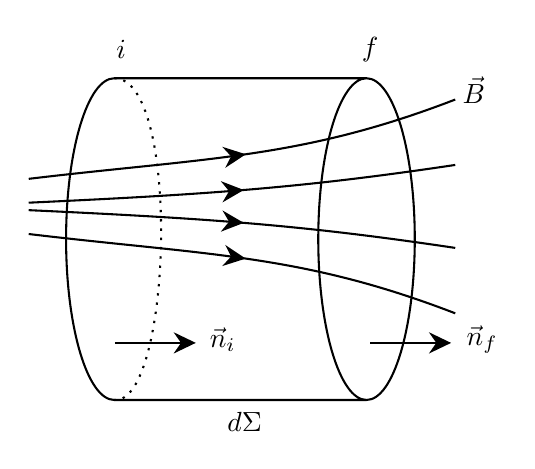
\begin{tikzpicture}[x=0.75pt,y=0.75pt,yscale=-1,xscale=1]
	%uncomment if require: \path (0,300); %set diagram left start at 0, and has height of 300

	%Curve Lines [id:da7344319235731953] 
	\draw    (212.5,118.96) .. controls (299.03,108.63) and (343.83,109.35) .. (418,80.75) ;
	\draw [shift={(317.06,107.12)}, rotate = 531.99] [fill={rgb, 255:red, 0; green, 0; blue, 0 }  ][line width=0.08]  [draw opacity=0] (10.72,-5.15) -- (0,0) -- (10.72,5.15) -- (7.12,0) -- cycle    ;
	%Curve Lines [id:da6735212516716587] 
	\draw    (212.5,145.54) .. controls (299.03,155.87) and (343.83,155.15) .. (418,183.75) ;
	\draw [shift={(317.06,157.38)}, rotate = 188.01] [fill={rgb, 255:red, 0; green, 0; blue, 0 }  ][line width=0.08]  [draw opacity=0] (10.72,-5.15) -- (0,0) -- (10.72,5.15) -- (7.12,0) -- cycle    ;
	%Curve Lines [id:da38088005125071667] 
	\draw    (212.5,130.45) .. controls (299.03,126.44) and (343.83,123.36) .. (418,112.26) ;
	\draw [shift={(316.12,124.33)}, rotate = 535.4] [fill={rgb, 255:red, 0; green, 0; blue, 0 }  ][line width=0.08]  [draw opacity=0] (10.72,-5.15) -- (0,0) -- (10.72,5.15) -- (7.12,0) -- cycle    ;
	%Curve Lines [id:da8905412173196354] 
	\draw    (212.5,134.05) .. controls (299.03,138.06) and (343.83,141.14) .. (418,152.24) ;
	\draw [shift={(316.12,140.17)}, rotate = 184.6] [fill={rgb, 255:red, 0; green, 0; blue, 0 }  ][line width=0.08]  [draw opacity=0] (10.72,-5.15) -- (0,0) -- (10.72,5.15) -- (7.12,0) -- cycle    ;
	%Straight Lines [id:da138108608465088] 
	\draw    (377,198) -- (413,198) ;
	\draw [shift={(416,198)}, rotate = 180] [fill={rgb, 255:red, 0; green, 0; blue, 0 }  ][line width=0.08]  [draw opacity=0] (10.72,-5.15) -- (0,0) -- (10.72,5.15) -- (7.12,0) -- cycle    ;
	%Shape: Can [id:dp8550992483460775] 
	\draw   (375.25,225.5) -- (253.75,225.5) .. controls (240.91,225.5) and (230.5,190.8) .. (230.5,148) .. controls (230.5,105.2) and (240.91,70.5) .. (253.75,70.5) -- (375.25,70.5) .. controls (388.09,70.5) and (398.5,105.2) .. (398.5,148) .. controls (398.5,190.8) and (388.09,225.5) .. (375.25,225.5) .. controls (362.41,225.5) and (352,190.8) .. (352,148) .. controls (352,105.2) and (362.41,70.5) .. (375.25,70.5) ;
	%Curve Lines [id:da5252519670188107] 
	\draw  [dash pattern={on 0.84pt off 2.51pt}]  (253.75,70.5) .. controls (286,70.25) and (281.5,227.75) .. (253.75,225.5) ;
	%Straight Lines [id:da7264894374138775] 
	\draw    (254,198) -- (290,198) ;
	\draw [shift={(293,198)}, rotate = 180] [fill={rgb, 255:red, 0; green, 0; blue, 0 }  ][line width=0.08]  [draw opacity=0] (10.72,-5.15) -- (0,0) -- (10.72,5.15) -- (7.12,0) -- cycle    ;

	% Text Node
	\draw (431,196.5) node    {$\vec{n}_{f}$};
	% Text Node
	\draw (427,76) node    {$\vec{B}$};
	% Text Node
	\draw (257,56.5) node    {$i$};
	% Text Node
	\draw (377,56.5) node    {$f$};
	% Text Node
	\draw (306,196.5) node    {$\vec{n}_{i}$};
	% Text Node
	\draw (316.5,236) node    {$d\Sigma $};

	\end{tikzpicture}
\end{figure}
\FloatBarrier

Se consideriamo la superficie chiusa $\Sigma$ data dall'unione di $ \Sigma_i  $ e $ \Sigma_f  $ e $ d\Sigma  $ e calcoliamo il flusso del campo attraverso tale superficie, dal momento che $ \text{div}\vec{B} =0 $:

\[
	\Phi_{\Sigma}(\vec{B}) = 0 = d\Phi_{d\Sigma} + \Phi_f - \Phi_i
\]
$\Phi_{\Sigma}(\vec{B})$ variazione di flusso magnetico concatenato al circuito.\\
$\Phi_f$ flusso concatenato al circuito nella posizione finale.\\
$\Phi_i$ flusso concatenato al circuito nella posizione iniziale.\\\\
La variazione di flusso attraverso la spira vale dunque:

\begin{gather*}
	d\Phi = \Phi_f-\Phi_i= -d\Phi_{d\Sigma} \\
	f_i = \frac{d\Phi_{d\Sigma}}{dt} = - \frac{d\Phi}{dt}
\end{gather*}

Se $ \Phi_f = \Phi_i $ non si ha variazione di flusso e non c'è quindi $fem$. È il caso di un campo magnetico uniforme.
Quando un circuito si muove rispetto alla sorgente di campo magnetico, compare la forza elettromotrice causata dalla forza di Lorentz. L'interpretazione è semplice: le forze di Lorentz mettono in moto le cariche.

Soffermiamoci sul caso di una sorgente di campo che si sposta rispetto al circuito fermo. Anche in questo caso le cariche saranno messe in moto: sperimentalmente si osserva infatti una corrente indotta. Non possiamo più parlare però di forze di Lorentz perché all'inizio le cariche sono ferme. Ci si può salvare grazie al principio di relatività di Galileo. Se ci poniamo in un sistema di riferimento che viaggia con il magnete, dato che nei due sistemi di riferimento dobbiamo osservare gli stessi effetti che avremmo se il magnete fosse fermo ed il circuito in moto, nel sistema solidale con il magente dobbiamo osservare una forza di Lorentz. Le due situazioni in figura diventano allora equivalenti.

\begin{figure}[htpb]
	\centering

	\tikzset{every picture/.style={line width=0.75pt}} %set default line width to 0.75pt        

	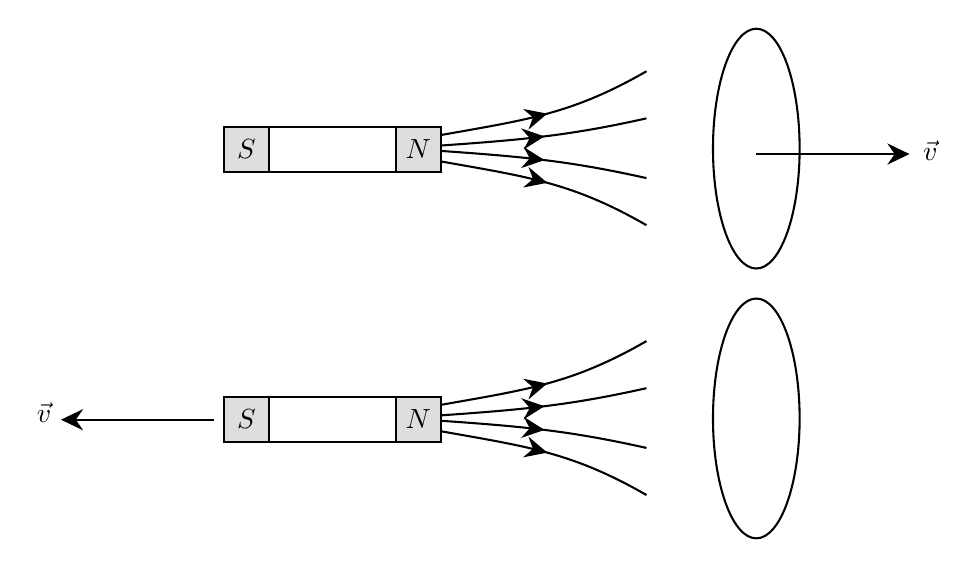
\begin{tikzpicture}[x=0.75pt,y=0.75pt,yscale=-1,xscale=1]
	%uncomment if require: \path (0,300); %set diagram left start at 0, and has height of 300

	%Shape: Rectangle [id:dp4576580186476005] 
	\draw   (158.62,73.56) -- (219.74,73.56) -- (219.74,95.18) -- (158.62,95.18) -- cycle ;
	%Shape: Rectangle [id:dp884221839198301] 
	\draw  [fill={rgb, 255:red, 222; green, 222; blue, 222 }  ,fill opacity=1 ] (219.74,73.56) -- (241.36,73.56) -- (241.36,95.18) -- (219.74,95.18) -- cycle ;
	%Shape: Rectangle [id:dp6940229120054398] 
	\draw  [fill={rgb, 255:red, 222; green, 222; blue, 222 }  ,fill opacity=1 ] (137,73.56) -- (158.62,73.56) -- (158.62,95.18) -- (137,95.18) -- cycle ;
	%Curve Lines [id:da7170417180295956] 
	\draw    (241.36,77.48) .. controls (283.1,70.04) and (304.72,67.32) .. (340.5,46.73) ;
	\draw [shift={(292.71,67.16)}, rotate = 525.38] [fill={rgb, 255:red, 0; green, 0; blue, 0 }  ][line width=0.08]  [draw opacity=0] (10.72,-5.15) -- (0,0) -- (10.72,5.15) -- (7.12,0) -- cycle    ;
	%Curve Lines [id:da2354299102413986] 
	\draw    (241.36,90.15) .. controls (283.1,97.59) and (304.72,100.31) .. (340.5,120.9) ;
	\draw [shift={(292.71,100.47)}, rotate = 194.62] [fill={rgb, 255:red, 0; green, 0; blue, 0 }  ][line width=0.08]  [draw opacity=0] (10.72,-5.15) -- (0,0) -- (10.72,5.15) -- (7.12,0) -- cycle    ;
	%Curve Lines [id:da6237417554819333] 
	\draw    (241.36,82.52) .. controls (283.1,79.63) and (304.72,77.41) .. (340.5,69.42) ;
	\draw [shift={(291.35,78.11)}, rotate = 533.3299999999999] [fill={rgb, 255:red, 0; green, 0; blue, 0 }  ][line width=0.08]  [draw opacity=0] (10.72,-5.15) -- (0,0) -- (10.72,5.15) -- (7.12,0) -- cycle    ;
	%Curve Lines [id:da42834637232751094] 
	\draw    (241.36,85.11) .. controls (283.1,88) and (304.72,90.22) .. (340.5,98.21) ;
	\draw [shift={(291.35,89.52)}, rotate = 186.67] [fill={rgb, 255:red, 0; green, 0; blue, 0 }  ][line width=0.08]  [draw opacity=0] (10.72,-5.15) -- (0,0) -- (10.72,5.15) -- (7.12,0) -- cycle    ;
	%Shape: Ellipse [id:dp569553660133667] 
	\draw   (372.55,84) .. controls (372.55,52.09) and (381.9,26.23) .. (393.42,26.23) .. controls (404.95,26.23) and (414.29,52.09) .. (414.29,84) .. controls (414.29,115.91) and (404.95,141.77) .. (393.42,141.77) .. controls (381.9,141.77) and (372.55,115.91) .. (372.55,84) -- cycle ;
	%Straight Lines [id:da6756468793205106] 
	\draw    (393.42,86.61) -- (464.22,86.61) ;
	\draw [shift={(467.22,86.61)}, rotate = 180] [fill={rgb, 255:red, 0; green, 0; blue, 0 }  ][line width=0.08]  [draw opacity=0] (10.72,-5.15) -- (0,0) -- (10.72,5.15) -- (7.12,0) -- cycle    ;
	%Shape: Rectangle [id:dp33213827151315334] 
	\draw   (158.62,203.56) -- (219.74,203.56) -- (219.74,225.18) -- (158.62,225.18) -- cycle ;
	%Shape: Rectangle [id:dp6552487363357307] 
	\draw  [fill={rgb, 255:red, 222; green, 222; blue, 222 }  ,fill opacity=1 ] (219.74,203.56) -- (241.36,203.56) -- (241.36,225.18) -- (219.74,225.18) -- cycle ;
	%Shape: Rectangle [id:dp8652540665212969] 
	\draw  [fill={rgb, 255:red, 222; green, 222; blue, 222 }  ,fill opacity=1 ] (137,203.56) -- (158.62,203.56) -- (158.62,225.18) -- (137,225.18) -- cycle ;
	%Curve Lines [id:da928852271271053] 
	\draw    (241.36,207.48) .. controls (283.1,200.04) and (304.72,197.32) .. (340.5,176.73) ;
	\draw [shift={(292.71,197.16)}, rotate = 525.38] [fill={rgb, 255:red, 0; green, 0; blue, 0 }  ][line width=0.08]  [draw opacity=0] (10.72,-5.15) -- (0,0) -- (10.72,5.15) -- (7.12,0) -- cycle    ;
	%Curve Lines [id:da07363356769513385] 
	\draw    (241.36,220.15) .. controls (283.1,227.59) and (304.72,230.31) .. (340.5,250.9) ;
	\draw [shift={(292.71,230.47)}, rotate = 194.62] [fill={rgb, 255:red, 0; green, 0; blue, 0 }  ][line width=0.08]  [draw opacity=0] (10.72,-5.15) -- (0,0) -- (10.72,5.15) -- (7.12,0) -- cycle    ;
	%Curve Lines [id:da3642152110945718] 
	\draw    (241.36,212.52) .. controls (283.1,209.63) and (304.72,207.41) .. (340.5,199.42) ;
	\draw [shift={(291.35,208.11)}, rotate = 533.3299999999999] [fill={rgb, 255:red, 0; green, 0; blue, 0 }  ][line width=0.08]  [draw opacity=0] (10.72,-5.15) -- (0,0) -- (10.72,5.15) -- (7.12,0) -- cycle    ;
	%Curve Lines [id:da628470651353888] 
	\draw    (241.36,215.11) .. controls (283.1,218) and (304.72,220.22) .. (340.5,228.21) ;
	\draw [shift={(291.35,219.52)}, rotate = 186.67] [fill={rgb, 255:red, 0; green, 0; blue, 0 }  ][line width=0.08]  [draw opacity=0] (10.72,-5.15) -- (0,0) -- (10.72,5.15) -- (7.12,0) -- cycle    ;
	%Shape: Ellipse [id:dp0488916567302462] 
	\draw   (372.55,214) .. controls (372.55,182.09) and (381.9,156.23) .. (393.42,156.23) .. controls (404.95,156.23) and (414.29,182.09) .. (414.29,214) .. controls (414.29,245.91) and (404.95,271.77) .. (393.42,271.77) .. controls (381.9,271.77) and (372.55,245.91) .. (372.55,214) -- cycle ;
	%Straight Lines [id:da9571130691953209] 
	\draw    (61.42,214.61) -- (132.22,214.61) ;
	\draw [shift={(58.42,214.61)}, rotate = 0] [fill={rgb, 255:red, 0; green, 0; blue, 0 }  ][line width=0.08]  [draw opacity=0] (10.72,-5.15) -- (0,0) -- (10.72,5.15) -- (7.12,0) -- cycle    ;

	% Text Node
	\draw (147.81,84.37) node    {$S$};
	% Text Node
	\draw (230.55,84.37) node    {$N$};
	% Text Node
	\draw (477.28,85.12) node    {$\vec{v}$};
	% Text Node
	\draw (147.81,214.37) node    {$S$};
	% Text Node
	\draw (230.55,214.37) node    {$N$};
	% Text Node
	\draw (50.28,211.12) node    {$\vec{v}$};

	\end{tikzpicture}
\end{figure}
\FloatBarrier

Se vogliamo rimanere sullo stesso SI (quello solidale al circuito), nel secondo caso non possiamo parlare di forza di Lorentz. Possiamo solo interpretare la situazione dicendo che a causa della variazione di flusso di campo magnetico nel circuito si introduce un campo elettrico.

Abbiamo visto una legge di tipo integrale. Vediamo se esiste un equivalente locale della \textbf{legge di Faraday-Neumann-Lenz}. Immaginiamo di avere la solita situazione con $\gamma$, $\Sigma$ ed $\vec{n}$ in cui è presente un campo magnetico variabile nel tempo. Secondo questa legge ci aspettiamo che lungo il circuito si indica una $fem$ pari a:

\[
	-\frac{d\Phi_{\Sigma}(\vec{B} )}{dt}
\]

Possiamo portare la derivata dentro all'integrale e scrivere, usando anche il teorema di Stokes

\begin{equation*}
	\begin{aligned}
		\oint_{\gamma} \vec{E} \cdot d\vec{l} &= - \frac{d}{dt} \underbrace{\int_{\Sigma}\vec{B} \cdot \vec{n}\,dS}_{\Phi_{\Sigma}(\vec{B} )} = - \int_{\Sigma}\left( \frac{\partial \vec{B}}{\partial t}  \right) \cdot \vec{n} \,dS \\
		\oint_{\gamma} \vec{E} \cdot d\vec{l} &= \int_{\Sigma}(\text{rot}\vec{E} ) \cdot \vec{n} \,dS \qquad \implies \boxed{\text{rot}\vec{E} = - \frac{\partial \vec{B}}{\partial t}}
	\end{aligned}
\end{equation*}

Se i campi magnetici non variano nel tempo, torniamo alla situazione dei campi elettrostatici conservativi. Se c'è un campo magnetico variabile nel tempo, il campo elettrico diventa non conservativo, perché deve essere in grado di porre delle cariche in moto in un circuito.

\[
	\vec{\nabla} \cdot [\vec{\nabla} \times \vec{E} ] = 0 = \vec{\nabla} \cdot \left[ -\frac{\partial \vec{B}}{\partial t}  \right] = -\frac{\partial}{\partial t} \vec{\nabla} \cdot \vec{B}  \implies  \vec{\nabla} \cdot \vec{B} \quad \text{costante}
\]

Inoltre, in tal caso, la derivata è diversa da zero, quindi il rotore del campo è non nullo e automaticamente esiste un campo elettrico, anche in assenza di cariche. C'è un legame fortissimo fra campi elettrici e campi magnetici

Identità operatoriale: L'espressione Wb= Vs si può ricavare dalla legge di Faraday

\[
	[f_i] = \frac{[\Phi ]}{[T]} \qquad (V)=\frac{(Wb)}{(S)}
\]

Supponiamo di trovarci in una regione dello spazio in cui sono presenti delle cariche elettriche e dei circuiti con correnti variabili nel tempo. Una parte del campo elettrico sarà generato da $Q$, un'altra generata dai campi magnetici variabili nel tempo. In questo caso il campo elettrico potrebbe avere una espressione più complessa.
Nel caso stazionario vale la legge: $ \vec{E} = -\vec{\nabla} V $.
Avevamo poi espresso il campo $\vec{B}$ come rotore del potenziale vettore $\vec{A}$.

\begin{equation*}
	\begin{aligned}
		\vec{B} =\text{rot}\vec{A} \qquad \text{rot}\vec{E} &= - \frac{\partial \vec{B}}{\partial t} \\
		\text{rot}\vec{E} &= - \frac{\partial \text{rot}\vec{A}}{\partial t} = \text{rot}\left(-\frac{\partial \vec{A}}{\partial t} \right)
	\end{aligned}
\end{equation*}

Quindi $ \vec{E} = - \frac{\partial \vec{A}}{\partial t}  $
L'espressione più generale che lega i campi elettrici è allora questa:

\[
	\boxed{\vec{E} = - \vec{\nabla} V - \frac{\partial \vec{A}}{\partial t}}
\]

Usiamo il potenziale vettore per descrivere la parte di campo elettrico legata ai campi magnetici variabili

\section{Autoinduzione}

Abbiamo messo in evidenza che il campo magnetico generato dalla corrente che percorre un circuito dia luogo ad un flusso magnetico attraverso il circuito stesso, il cosiddetto autoflusso, che risulta proporzionale alla corrente i tramite il coefficiente di autoinduzione $L$, che dipende dalla forma geometrica del circuito e dalla permeabilità magnetica del mezzo in cui il circuito è immerso.

\begin{figure}[htpb]
	\centering

	% Pattern Info
	 
	\tikzset{
	pattern size/.store in=\mcSize, 
	pattern size = 5pt,
	pattern thickness/.store in=\mcThickness, 
	pattern thickness = 0.3pt,
	pattern radius/.store in=\mcRadius, 
	pattern radius = 1pt}
	\makeatletter
	\pgfutil@ifundefined{pgf@pattern@name@_jmy2ayvgh}{
	\pgfdeclarepatternformonly[\mcThickness,\mcSize]{_jmy2ayvgh}
	{\pgfqpoint{0pt}{0pt}}
	{\pgfpoint{\mcSize+\mcThickness}{\mcSize+\mcThickness}}
	{\pgfpoint{\mcSize}{\mcSize}}
	{
	\pgfsetcolor{\tikz@pattern@color}
	\pgfsetlinewidth{\mcThickness}
	\pgfpathmoveto{\pgfqpoint{0pt}{0pt}}
	\pgfpathlineto{\pgfpoint{\mcSize+\mcThickness}{\mcSize+\mcThickness}}
	\pgfusepath{stroke}
	}}
	\makeatother
	\tikzset{every picture/.style={line width=0.75pt}} %set default line width to 0.75pt        

	\begin{tikzpicture}[x=0.75pt,y=0.75pt,yscale=-1,xscale=1]
	%uncomment if require: \path (0,300); %set diagram left start at 0, and has height of 300

	%Shape: Ellipse [id:dp24672730295208045] 
	\draw  [pattern=_jmy2ayvgh,pattern size=6pt,pattern thickness=0.75pt,pattern radius=0pt, pattern color={rgb, 255:red, 222; green, 222; blue, 222}] (192.63,146.83) .. controls (192.71,111.3) and (238.4,82.6) .. (294.68,82.74) .. controls (350.95,82.87) and (396.5,111.79) .. (396.41,147.33) .. controls (396.33,182.87) and (350.64,211.56) .. (294.36,211.43) .. controls (238.09,211.29) and (192.54,182.37) .. (192.63,146.83) -- cycle ;
	\draw   (291.47,205.66) -- (302.39,211.6) -- (291.09,216.78) ;
	%Straight Lines [id:da9427327099690423] 
	\draw    (294.52,147.08) -- (294.78,40.26) ;
	\draw [shift={(294.79,37.26)}, rotate = 450.14] [fill={rgb, 255:red, 0; green, 0; blue, 0 }  ][line width=0.08]  [draw opacity=0] (10.72,-5.15) -- (0,0) -- (10.72,5.15) -- (7.12,0) -- cycle    ;
	%Curve Lines [id:da49715380719001945] 
	\draw    (200,244) .. controls (250.5,163) and (263.5,86) .. (219.5,33) ;
	\draw [shift={(243.62,138.9)}, rotate = 460.89] [fill={rgb, 255:red, 0; green, 0; blue, 0 }  ][line width=0.08]  [draw opacity=0] (10.72,-5.15) -- (0,0) -- (10.72,5.15) -- (7.12,0) -- cycle    ;
	%Curve Lines [id:da30757913025138395] 
	\draw    (348,256) .. controls (316.5,163) and (313.5,87) .. (384.5,44) ;
	\draw [shift={(327.05,140.01)}, rotate = 452.21] [fill={rgb, 255:red, 0; green, 0; blue, 0 }  ][line width=0.08]  [draw opacity=0] (10.72,-5.15) -- (0,0) -- (10.72,5.15) -- (7.12,0) -- cycle    ;

	% Text Node
	\draw (406,160.5) node    {$\gamma $};
	% Text Node
	\draw (313,41) node    {$\vec{n}$};
	% Text Node
	\draw (374,140.5) node    {$\Sigma $};
	% Text Node
	\draw (291.5,229) node    {$I( t)$};
	% Text Node
	\draw (399.3,38.08) node    {$\vec{B}$};

	\end{tikzpicture}
\end{figure}
\FloatBarrier

La nozione di autoflusso acquista particolare importanza quando la corrente nel circuito non è costante nel tempo (oppure quando viene variata la sua forma).

\[
	\Phi_{\Sigma}(\vec{B}) = \int_{\Sigma}\vec{B} \cdot \vec{n} \,dS >0  \qquad \Phi_{\Sigma}(\vec{B}) = L\cdot I(t)
\]

Il flusso concatenato con il circuito cambia nel tempo e nel circuito compare una $fem$ indotta che con i suoi effetti tende ad opporsi alla variazione che l'ha generata. Tale $fem$ si calcola come:

\[
	f_i = - \frac{d\Phi_{\Sigma}(\vec{B} )}{dt} = -\frac{d}{dt}(L\,I) = -L\,\frac{d}{dt}I
\]

In caso di materiali dia e para magnetici, $L$ può essere portato fuori dalla derivata.
Tale risultato fornisce operativamente la definizione del coefficiente $L$ di un qualsiasi circuito, purché rigido, immerso in un mezzo qualunque. Si deve supporre però che le variazioni di corrente non siano così rapide da avvenire in un tempo paragonabile a quello impiegato dalla luce a percorrere la dimensione tipica del circuito, perché in tal caso la corrente non avrebbe più lo stesso valore su diverse sezioni del circuito. Il coefficiente di autoinduzione di un circuito viene comunemente indicato con il termine \emph{induttanza}. Un circuito con induttanza non nulla si dice induttivo.
Molto spesso si rappresenta l'effetto di induzione elettromagnetica sul circuito immaginando che questo effetto sia legato ad un oggetto chiamato \emph{induttore}, ad esempio perché il filo conduttore è avvolto così da formare un solenoide.

Ad ogni modo, la presenza di un induttore in un circuito impedisce alla corrente di aumentare o diminuire istantaneamente in quanto la variazione genera una $fem$ che si oppone alla variazione stessa. Esaminiamo il caso di un circuito $RLC$ serie, costituito da un generatore di $fem$ e resistenza interna trascurabile, da un induttore con induttanza $L$ e da un resistore di resistenza $R$. Le variazioni di corrente sono causate inizialmente dall'apertura e dalla chiusura dell'interruttore $T$.

\begin{figure}[htpb]
	\centering

	\tikzset{every picture/.style={line width=0.75pt}} %set default line width to 0.75pt        

	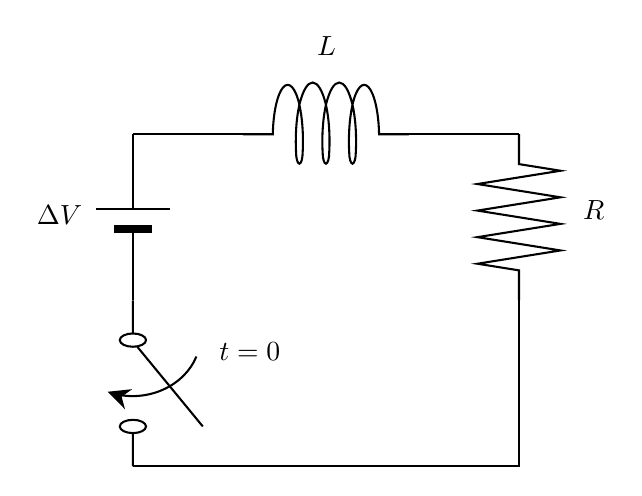
\begin{tikzpicture}[x=0.75pt,y=0.75pt,yscale=-1,xscale=1]
	%uncomment if require: \path (0,300); %set diagram left start at 0, and has height of 300

	%Shape: Inductor (Air Core) [id:dp1811299889194351] 
	\draw   (220,77) -- (234.4,77) .. controls (234.61,66.49) and (236.61,57.51) .. (239.43,54.37) .. controls (242.26,51.23) and (245.35,54.57) .. (247.2,62.79) .. controls (248.63,69.2) and (249.21,77.48) .. (248.8,85.53) .. controls (248.8,88.67) and (248.08,91.21) .. (247.2,91.21) .. controls (246.32,91.21) and (245.6,88.67) .. (245.6,85.53) .. controls (245.19,77.48) and (245.77,69.2) .. (247.2,62.79) .. controls (248.86,55.96) and (251.18,52.09) .. (253.6,52.09) .. controls (256.02,52.09) and (258.34,55.96) .. (260,62.79) .. controls (261.43,69.2) and (262.01,77.48) .. (261.6,85.53) .. controls (261.6,88.67) and (260.88,91.21) .. (260,91.21) .. controls (259.12,91.21) and (258.4,88.67) .. (258.4,85.53) .. controls (257.99,77.48) and (258.57,69.2) .. (260,62.79) .. controls (261.66,55.96) and (263.98,52.09) .. (266.4,52.09) .. controls (268.82,52.09) and (271.14,55.96) .. (272.8,62.79) .. controls (274.23,69.2) and (274.81,77.48) .. (274.4,85.53) .. controls (274.4,88.67) and (273.68,91.21) .. (272.8,91.21) .. controls (271.92,91.21) and (271.2,88.67) .. (271.2,85.53) .. controls (270.79,77.48) and (271.37,69.2) .. (272.8,62.79) .. controls (274.65,54.57) and (277.74,51.23) .. (280.57,54.37) .. controls (283.39,57.51) and (285.39,66.49) .. (285.6,77) -- (300,77) ;
	%Shape: Resistor [id:dp6080934326111651] 
	\draw   (353,77) -- (353,91.4) -- (373,94.6) -- (333,101) -- (373,107.4) -- (333,113.8) -- (373,120.2) -- (333,126.6) -- (373,133) -- (333,139.4) -- (353,142.6) -- (353,157) ;
	%Shape: Battery [id:dp6120838199192846] 
	\draw  [fill={rgb, 255:red, 0; green, 0; blue, 0 }  ,fill opacity=1 ] (167,157) -- (167,121) (149.33,113) -- (184.67,113) (167,113) -- (167,77) (158.17,124.2) -- (158.17,121) -- (175.83,121) -- (175.83,124.2) -- (158.17,124.2) -- cycle ;
	%Shape: Simple Switch [id:dp7474022825810089] 
	\draw   (167,157) -- (167,173) (167,221) -- (167,237) (169.11,179.4) -- (200.68,217.8) (167,214.6) .. controls (170.49,214.6) and (173.32,216.03) .. (173.32,217.8) .. controls (173.32,219.57) and (170.49,221) .. (167,221) .. controls (163.51,221) and (160.68,219.57) .. (160.68,217.8) .. controls (160.68,216.03) and (163.51,214.6) .. (167,214.6) -- cycle (167,173) .. controls (170.49,173) and (173.32,174.43) .. (173.32,176.2) .. controls (173.32,177.97) and (170.49,179.4) .. (167,179.4) .. controls (163.51,179.4) and (160.68,177.97) .. (160.68,176.2) .. controls (160.68,174.43) and (163.51,173) .. (167,173) -- cycle ;
	%Straight Lines [id:da3068766871707447] 
	\draw    (167,77) -- (220,77) ;
	%Curve Lines [id:da6227103172248754] 
	\draw    (197.58,184.12) .. controls (191.81,198.19) and (174.26,206.48) .. (157.48,201.92) ;
	\draw [shift={(154.84,201.09)}, rotate = 379.61] [fill={rgb, 255:red, 0; green, 0; blue, 0 }  ][line width=0.08]  [draw opacity=0] (10.72,-5.15) -- (0,0) -- (10.72,5.15) -- (7.12,0) -- cycle    ;
	%Straight Lines [id:da4133366237660214] 
	\draw    (300,77) -- (353,77) ;
	%Straight Lines [id:da9569159529670197] 
	\draw    (167,237) -- (353.33,237) ;
	%Straight Lines [id:da2964493224854299] 
	\draw    (353,237) -- (353,157) ;

	% Text Node
	\draw (260.33,34.67) node    {$L$};
	% Text Node
	\draw (389,113.33) node    {$R$};
	% Text Node
	\draw (131.67,116) node    {$\Delta V$};
	% Text Node
	\draw (223.33,181.67) node    {$t=0$};

	\end{tikzpicture}
\end{figure}
\FloatBarrier

Chiediamoci cosa succede quando in $T=0$ chiudiamo il circuito.
In assenza di fenomeni di induzione elettromagnetica, ci aspetteremmo che alla chiusura abbiamo un corrente istantanea calcolabile con la legge di Ohm. Questo nella pratica non accade. Nel momento in cui chiudiamo un circuito, esso comincia a produrre un campo magnetico. Apparirà una forza elettromotrice indotta che si oppone all'aumento di $\vec{B}$. Possiamo dire che:

\begin{gather*}
	\Delta V + f_i = RI \\
	\Delta V \underbrace{-L \frac{dI}{dt}}_{f_i} = RI \\
	- L \frac{dI}{dt} = RI - \Delta V \\
	- \underbrace{\frac{L}{R}}_{\tau} \frac{dI}{dt} = I - \underbrace{\frac{\Delta V}{R}}_{I_{\infty}} \\
	-\tau \frac{dI}{dt} = I - I_{\infty} \\
	- \frac{\tau}{dt} = \frac{I-I_{\infty}}{dI} \\
	- \int \frac{dt}{\tau} = \int \frac{dI}{I-I_{\infty}} \\
	-\frac{t}{\tau} = [\log (I-I_{\infty})]_0^{I(t)} = \log (I(t)-I_{\infty})-\log (-I_{\infty} ) \\
	-\frac{t}{\tau} = \log \frac{I(t)-I_{\infty}}{-I_{\infty}} \\
	e^{-t/\tau} = \frac{I(t)-I_{\infty}}{-I_{\infty}} \\
	I_{\infty}-I_{\infty}e^{-t/\tau} = I(t) \implies \boxed{I(t)=I_{\infty}(1-e^{-t/\tau} )}
\end{gather*}

All'istante iniziale compare subito una $fem$ che si oppone alla causa che la sta generando. All'inizio tale forza è talmente intensa da dare corrente iniziale pari a zero. Più avanti vince il generatore e la corrente sale lentamente.

\begin{figure}[htpb]
	\centering

	\tikzset{every picture/.style={line width=0.75pt}} %set default line width to 0.75pt        

	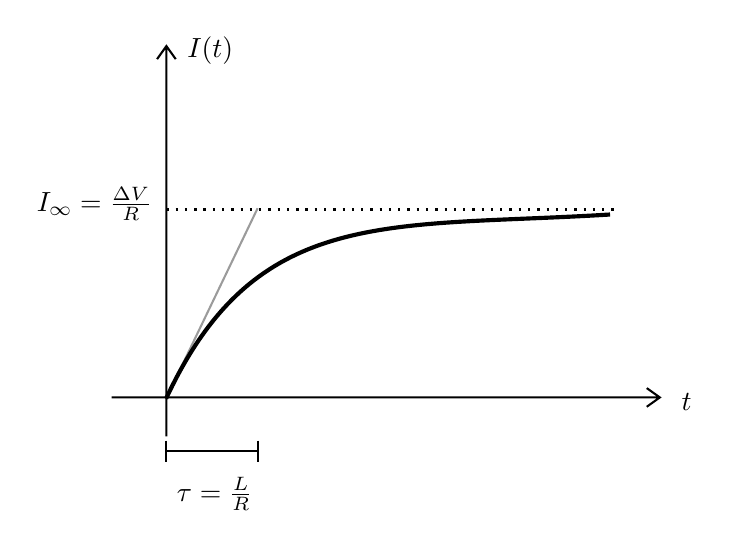
\begin{tikzpicture}[x=0.75pt,y=0.75pt,yscale=-0.9,xscale=0.9]
	%uncomment if require: \path (0,355); %set diagram left start at 0, and has height of 355

	%Straight Lines [id:da45293825265519105] 
	\draw [color={rgb, 255:red, 155; green, 155; blue, 155 }  ,draw opacity=1 ]   (232.35,243.2) -- (281.33,141.33) ;
	%Shape: Axis 2D [id:dp5077172548790807] 
	\draw  (203.15,242.6) -- (496.65,242.6)(232.5,54.5) -- (232.5,263.5) (489.65,237.6) -- (496.65,242.6) -- (489.65,247.6) (227.5,61.5) -- (232.5,54.5) -- (237.5,61.5)  ;
	%Straight Lines [id:da4075929645086587] 
	\draw  [dash pattern={on 0.84pt off 2.51pt}]  (232.5,142) -- (473,142) ;
	% Plotting does not support converting to Tikz
	%Curve Lines [id:da11473619874977481] 
	\draw [line width=1.5]    (232.35,243.2) .. controls (280.67,139.33) and (351.33,152) .. (470,144.67) ;
	%Straight Lines [id:da9117039057161145] 
	\draw    (232.5,271.33) -- (281.33,271.33) ;
	\draw [shift={(281.33,271.33)}, rotate = 180] [color={rgb, 255:red, 0; green, 0; blue, 0 }  ][line width=0.75]    (0,5.59) -- (0,-5.59)   ;
	\draw [shift={(232.5,271.33)}, rotate = 180] [color={rgb, 255:red, 0; green, 0; blue, 0 }  ][line width=0.75]    (0,5.59) -- (0,-5.59)   ;

	% Text Node
	\draw (256,57) node    {$I( t)$};
	% Text Node
	\draw (511,245) node    {$t$};
	% Text Node
	\draw (194,139) node    {$I_{\infty } =\frac{\Delta V}{R}$};
	% Text Node
	\draw (258.33,294.33) node    {$\tau =\frac{L}{R}$};

	\end{tikzpicture}
\end{figure}
\FloatBarrier

\textbf{Osservazione.} Notiamo che $ I(t) $ tende asintoticamente al valore di regime $ I_{\infty}=\frac{\Delta V}{R}  $ corrispondente alla legge di Ohm per le correnti costanti. Il raggiungimento di tale valore è legato alla costante di tempo.

\section{Energia magnetica}

La presenza di una $fem$ in un circuito implica, per definizione, un lavoro sulle cariche che costituiscono la corrente, positivo o negativo a seconda del segno della $fem$. Il lavoro $dt$ compiuto dal generatore per sostenere il moto delle cariche quando la corrente ha valore $I$ è dato da:

\[
	\underbrace{\Delta V = RI + L\frac{dI}{dt}}_{\text{moltiplico per}I\,dt} \implies \Delta V\,I\,dt = R\,I^2 dt + L\,I\,dI
\]

Questa espressione esprime il bilancio energetico del circuito. Il primo membro è il lavoro compiuto dal generatore per far circolare corrente nel circuito e trasformato in calore (effetto Joule). Il termine $L\,I\,dI$ è il lavoro speso contro la $fem$ di autoinduzione per far aumentare la corrente da $I$ a $I+dI$. Nell'intervallo di tempo in cui, a seguito della chiusura del circuito, la corrente passa da zero al valore $ I_{\infty}  $, il generatore oltre che al lavoro corrispondente all'effetto Joule deve spendere contro la $fem$ di autoinduzione il lavoro:

\[
	\mathcal{L}_i = \int d\mathcal{L}_i = \int_0^{I_{\infty}} L\,I\,dI = \left[ \frac{1}{2} L\,I^2  \right]_0^{I_{\infty}} = \frac{1}{2} L\,I_{\infty}^2
\]

Che non dipende dal modo in cui avviene la variazione di corrente, ma solo dal valore iniziale e finale. Possiamo interpretare questo lavoro come una energia magnetica che il circuito possiede. Avevamo parlato di una forma di energia analoga nel caso del campo elettrostatico del condensatore e avevamo definito una densità di energia per unità di volume. Ci si può chiedere se anche quest'altra energia magnetica sia visibile come un energia distribuita in tutto lo spazio in cui è presente il campo magnetico generato dal circuito. Dopotutto, l'espressione dell'energia magnetica suggerisce che essa sia legata al campo $\vec{B}$ e localizzabile nello spazio in cui tale campo esiste. Consideriamo un solenoide vuoto rettilineo infinito e su di esso un pezzo di lunghezza finita $L$.

\begin{figure}[htpb]
	\centering

	\tikzset{every picture/.style={line width=0.75pt}} %set default line width to 0.75pt        

	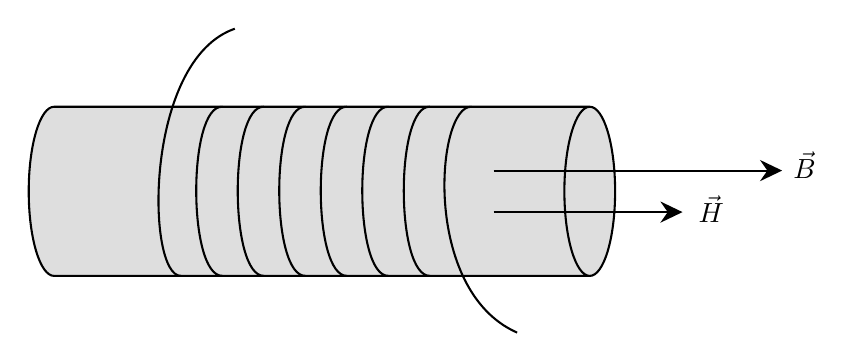
\begin{tikzpicture}[x=0.75pt,y=0.75pt,yscale=-1,xscale=1]
	%uncomment if require: \path (0,300); %set diagram left start at 0, and has height of 300

	%Shape: Can [id:dp7741966840400853] 
	\draw  [fill={rgb, 255:red, 222; green, 222; blue, 222 }  ,fill opacity=1 ] (406.81,187.5) -- (148.73,187.5) .. controls (141.97,187.5) and (136.5,169.26) .. (136.5,146.75) .. controls (136.5,124.24) and (141.97,106) .. (148.73,106) -- (406.81,106) .. controls (413.56,106) and (419.03,124.24) .. (419.03,146.75) .. controls (419.03,169.26) and (413.56,187.5) .. (406.81,187.5) .. controls (400.06,187.5) and (394.58,169.26) .. (394.58,146.75) .. controls (394.58,124.24) and (400.06,106) .. (406.81,106) ;
	%Curve Lines [id:da210960011768905] 
	\draw    (235.8,68.4) .. controls (191.8,83.6) and (193,187.6) .. (209.81,187.5) ;
	%Curve Lines [id:da8398771468545265] 
	\draw    (229.81,106) .. controls (213,105.2) and (213,187.6) .. (229.81,187.5) ;
	%Curve Lines [id:da4560936194642726] 
	\draw    (249.81,106) .. controls (233,105.2) and (233,187.6) .. (249.81,187.5) ;
	%Curve Lines [id:da5759943950482904] 
	\draw    (269.81,106) .. controls (253,105.2) and (253,187.6) .. (269.81,187.5) ;
	%Curve Lines [id:da7046738061237652] 
	\draw    (289.81,106) .. controls (273,105.2) and (273,187.6) .. (289.81,187.5) ;
	%Curve Lines [id:da5602030346503439] 
	\draw    (309.81,106) .. controls (293,105.2) and (293,187.6) .. (309.81,187.5) ;
	%Curve Lines [id:da16002715564423253] 
	\draw    (329.81,106) .. controls (313,105.2) and (313,187.6) .. (329.81,187.5) ;
	%Curve Lines [id:da19557435324446426] 
	\draw    (349.81,106) .. controls (333,105.2) and (325.4,194.4) .. (371.8,214.8) ;
	%Straight Lines [id:da3714557523081883] 
	\draw    (360.5,136.75) -- (496.5,136.75) ;
	\draw [shift={(499.5,136.75)}, rotate = 180] [fill={rgb, 255:red, 0; green, 0; blue, 0 }  ][line width=0.08]  [draw opacity=0] (10.72,-5.15) -- (0,0) -- (10.72,5.15) -- (7.12,0) -- cycle    ;
	%Straight Lines [id:da5351098831815313] 
	\draw    (360.5,156.75) -- (448.5,156.75) ;
	\draw [shift={(451.5,156.75)}, rotate = 180] [fill={rgb, 255:red, 0; green, 0; blue, 0 }  ][line width=0.08]  [draw opacity=0] (10.72,-5.15) -- (0,0) -- (10.72,5.15) -- (7.12,0) -- cycle    ;

	% Text Node
	\draw (510.3,134.08) node    {$\vec{B}$};
	% Text Node
	\draw (465.3,155.08) node    {$\vec{H}$};

	\end{tikzpicture}
\end{figure}
\FloatBarrier

Conosciamo l'area di sezione del solenoide $S$. Si produce a causa della corrente un campo magnetico al suo interno che sappiamo calcolare come:

\[
	B = \mu_0 n_s\,I \qquad H = n_s\,I
\]

Dobbiamo moltiplicare il flusso per il numero di spire.

\begin{align*}
	&L = \frac{\Phi_{\text{autoconcatenato}}(\vec{B})}{I} = \frac{B\,S\,N}{I} = \frac{\mu_0 n_s I\cdot S \cdot n_s\,l}{I} = \mu_0 n_s^2 S\,l \\
	&\boxed{U_m = \frac{1}{2} L\,I^2} = \frac{1}{2} (\mu_0 n_s^2 S\,l)\,I^2
\end{align*}

Notiamo che $S\,l$ è il volume contenuto all'interno di questa porzione di solenoide. Questa energia magnetica in effetti è proporzionale al suo volume. Ha senso definire una densità di energia magnetica per unità di volume come:

\[
	u_m = \frac{U_m}{\text{volume}} = \frac{U_m}{S\,l} = \frac{\frac{1}{2} (\mu_0 n_s^2 S\,l)\,I^2}{S\,l} = \frac{1}{2} \mu_0 n_s^2\,I^2
\]

Data la struttura di questa espressione, che dipende solo dal valore del campo magnetico e dalla permeabilità del mezzo (che è il vuoto) siamo portati a concludere che il risultato trovato valga sempre, nel vuoto, qualunque sia l'andamento del campo magnetico e la sorgente che lo genera. Possiamo riscrivere la densità di energia per unità di volume come:

\[
	u_m = \underbrace{\frac{1}{2} \mu_0 n_s^2\,I^2}_{\text{moltiplico e divido per}\mu_0} = \frac{1}{2} \frac{\mu_0^2 n_s^2\,I^2}{\mu_0} = \boxed{\frac{1}{2} \frac{B^2}{\mu_0} = u_m}
\]

Notiamo l'analogia con la struttura della densità di energia elettrostatica:

\[
	u_e = \frac{1}{2} \varepsilon_0 E^2
\]

L'energia magnetica potrà allora essere calcolata come:

\[
	U_m = \int_{\text{spazio}} u_m d\tau
\]

Vediamo cosa accade in presenza di materiali magnetici. Dobbiamo distinguere anche in questo caso i materiali dia e para magnetici da quelli ferromagnetici.
Immaginiamo che dentro il solenoide ci sia un materiale con una certa permeabilità magnetica $\mu_r$.

\begin{figure}[htpb]
	\centering

	\tikzset{every picture/.style={line width=0.75pt}} %set default line width to 0.75pt        

	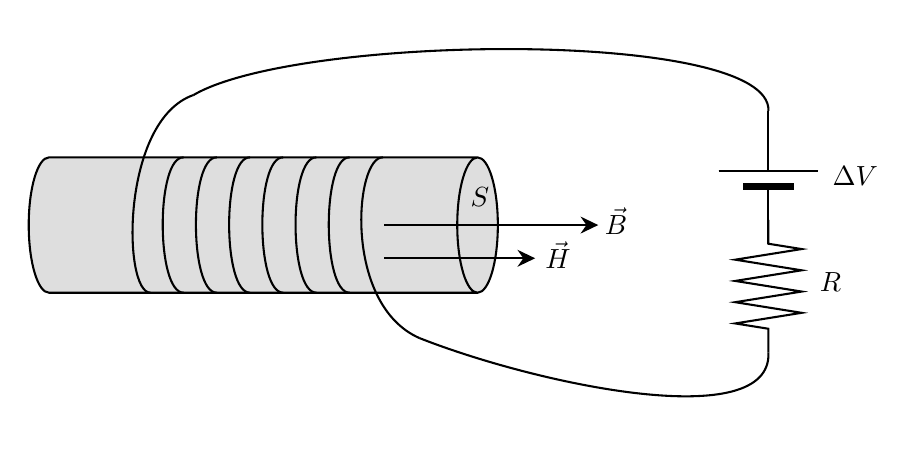
\begin{tikzpicture}[x=0.75pt,y=0.75pt,yscale=-0.8,xscale=0.8]
	%uncomment if require: \path (0,300); %set diagram left start at 0, and has height of 300

	%Shape: Can [id:dp3503983742611452] 
	\draw  [fill={rgb, 255:red, 222; green, 222; blue, 222 }  ,fill opacity=1 ] (326.81,197.5) -- (68.72,197.5) .. controls (61.97,197.5) and (56.5,179.26) .. (56.5,156.75) .. controls (56.5,134.24) and (61.97,116) .. (68.72,116) -- (326.81,116) .. controls (333.56,116) and (339.03,134.24) .. (339.03,156.75) .. controls (339.03,179.26) and (333.56,197.5) .. (326.81,197.5) .. controls (320.06,197.5) and (314.58,179.26) .. (314.58,156.75) .. controls (314.58,134.24) and (320.06,116) .. (326.81,116) ;
	%Curve Lines [id:da6125100454529431] 
	\draw    (155.8,78.4) .. controls (111.8,93.6) and (113,197.6) .. (129.81,197.5) ;
	%Curve Lines [id:da9453283806790904] 
	\draw    (149.81,116) .. controls (133,115.2) and (133,197.6) .. (149.81,197.5) ;
	%Curve Lines [id:da05294172617481241] 
	\draw    (169.81,116) .. controls (153,115.2) and (153,197.6) .. (169.81,197.5) ;
	%Curve Lines [id:da5691564596361309] 
	\draw    (189.81,116) .. controls (173,115.2) and (173,197.6) .. (189.81,197.5) ;
	%Curve Lines [id:da5246721629101647] 
	\draw    (209.81,116) .. controls (193,115.2) and (193,197.6) .. (209.81,197.5) ;
	%Curve Lines [id:da5701541332841926] 
	\draw    (229.81,116) .. controls (213,115.2) and (213,197.6) .. (229.81,197.5) ;
	%Curve Lines [id:da3391028947263257] 
	\draw    (249.81,116) .. controls (233,115.2) and (233,197.6) .. (249.81,197.5) ;
	%Curve Lines [id:da06860635740055199] 
	\draw    (269.81,116) .. controls (253,115.2) and (245.4,204.4) .. (291.8,224.8) ;
	%Straight Lines [id:da5282854737648179] 
	\draw    (270.5,156.75) -- (396.5,156.75) ;
	\draw [shift={(399.5,156.75)}, rotate = 180] [fill={rgb, 255:red, 0; green, 0; blue, 0 }  ][line width=0.08]  [draw opacity=0] (10.72,-5.15) -- (0,0) -- (10.72,5.15) -- (7.12,0) -- cycle    ;
	%Straight Lines [id:da26118252633211325] 
	\draw    (270.5,176.75) -- (358.5,176.75) ;
	\draw [shift={(361.5,176.75)}, rotate = 180] [fill={rgb, 255:red, 0; green, 0; blue, 0 }  ][line width=0.08]  [draw opacity=0] (10.72,-5.15) -- (0,0) -- (10.72,5.15) -- (7.12,0) -- cycle    ;
	%Shape: Battery [id:dp7697106590049856] 
	\draw  [fill={rgb, 255:red, 0; green, 0; blue, 0 }  ,fill opacity=1 ] (502,168) -- (502,132) (472,124) -- (532,124) (502,124) -- (502,88) (487,135.2) -- (487,132) -- (517,132) -- (517,135.2) -- (487,135.2) -- cycle ;
	%Shape: Resistor [id:dp3604906038927598] 
	\draw   (502,153.6) -- (502,168) -- (522,171.2) -- (482,177.6) -- (522,184) -- (482,190.4) -- (522,196.8) -- (482,203.2) -- (522,209.6) -- (482,216) -- (502,219.2) -- (502,233.6) ;
	%Curve Lines [id:da19416694906660026] 
	\draw    (502,88) .. controls (504,38.5) and (219,41.5) .. (155.8,78.4) ;
	%Curve Lines [id:da028991734151780246] 
	\draw    (502,233.6) .. controls (504,283.1) and (362,252.5) .. (291.8,224.8) ;

	% Text Node
	\draw (410.3,154.08) node    {$\vec{B}$};
	% Text Node
	\draw (375.3,175.08) node    {$\vec{H}$};
	% Text Node
	\draw (328.3,140.08) node    {$S$};
	% Text Node
	\draw (554.3,127.08) node    {$\Delta V$};
	% Text Node
	\draw (539.3,191.08) node    {$R$};

	\end{tikzpicture}
\end{figure}
\FloatBarrier

Colleghiamo un generatore reale al solenoide. Facendo aumentare la corrente da $0$ a $I$ il flusso concatenato alle spire cambia e nascerà una $fem$. La legge del circuito all'istante $t$ è:

\begin{equation*}
	\begin{aligned}
		\Delta V + f_i &= RI \\
		\Delta V - \frac{d\Phi (\vec{B})}{dt} &= RI \\
		\Delta V &= RI + \frac{d\Phi (\vec{B})}{dt} \\
	\end{aligned}
\end{equation*}

E il lavoro speso dal generatore è:

\[
	\underbrace{\Delta V\,I\,dt}_{\text{generatore}} = \underbrace{R\,I^2 dt}_{\text{effetto Joule}} + \underbrace{I\,d\Phi}_{\text{campo} \vec{B}}
\]

A sinistra abbiamo un termine legato al lavoro compiuto dal generatore. Il secondo è il lavoro speso per vincere l'effetto Joule. Il terzo è associato al lavoro speso per creare il campo magnetico all'interno del materiale. La variazione di flusso è:

\[
	\Phi (\vec{B}) = B\,S\,n_s\,l  \implies  d\Phi (\vec{B} ) = n_s\,S\,l\,dB
\]

Essa è legata alla variazione del campo $\vec{B}$. Pertanto il lavoro speso contro la $fem$ di autoinduzione è dato da

\[
	\mathcal{L}_i = \int d\mathcal{L}_i =\int I\,d\Phi = \int \underbrace{I n_s}_H\,dB\,\underbrace{S\,l}_{\tau} = \tau \int_0^{B_{\text{finale}}} H(B) \;dB
\]

E quindi l'energia magnetica per unità di volume è data da:\[
	\boxed{u_m = \int_0^{B_{\text{finale}}} H(B) \;dB}
\]

Possiamo scrivere $ \vec{H}  $ come

\[
	H = \frac{B}{\mu_0 \mu_r} \implies u_m = \int_0^{B_{\text{finale}}} \frac{B}{\mu_0 \mu_r} \;dB = \frac{1}{2} \frac{B^2_{\text{finale}}}{\mu_r \mu_0} = \frac{1}{2} \vec{B} \cdot \vec{H}
\]

Tale legge ha validità generale nei materiali diamagnetici e paramagnetici, mentre nei ferromagnetici si possono applicare solo in quelle situazioni in cui la permeabilità si può ritenere costante. Avevamo anche in questo caso trovato un espressione simile parlando di energia elettrostatica in presenza di dielettrici.

L'energia magnetica corrisponde al lavoro speso dal generatore per produrre il campo magnetico, nel vuoto e nei materiali, in aggiunta al lavoro speso per far circolare la corrente. Nei mezzi in cui vi è proporzionalità diretta fra $\vec{B}$ ed $\vec{H}$, i processi di magnetizzazione e smagnetizzazione avvengono reversibilmente. (Ci muoviamo lungo la stessa retta).

\begin{figure}[htpb]
	\centering

	\tikzset{every picture/.style={line width=0.75pt}} %set default line width to 0.75pt        

	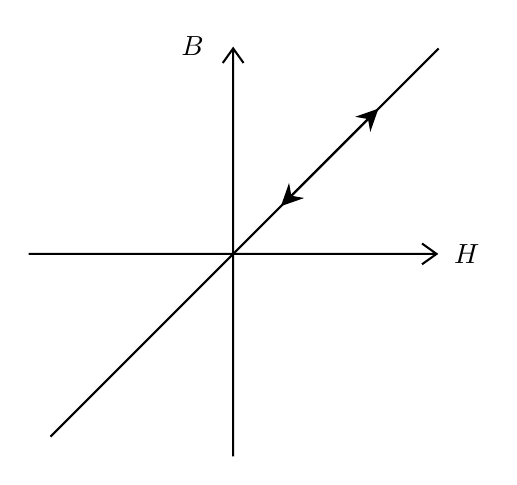
\begin{tikzpicture}[x=0.75pt,y=0.75pt,yscale=-1,xscale=1]
	%uncomment if require: \path (0,300); %set diagram left start at 0, and has height of 300

	%Shape: Axis 2D [id:dp5096057532745446] 
	\draw  (167,142) -- (363.5,142)(265.5,43) -- (265.5,239.5) (356.5,137) -- (363.5,142) -- (356.5,147) (260.5,50) -- (265.5,43) -- (270.5,50)  ;
	%Straight Lines [id:da5479025621943316] 
	\draw    (177.5,230) -- (364.5,43) ;
	%Straight Lines [id:da5756808453246931] 
	\draw    (290.62,116.88) -- (333.38,74.12) ;
	\draw [shift={(335.5,72)}, rotate = 495] [fill={rgb, 255:red, 0; green, 0; blue, 0 }  ][line width=0.08]  [draw opacity=0] (10.72,-5.15) -- (0,0) -- (10.72,5.15) -- (7.12,0) -- cycle    ;
	\draw [shift={(288.5,119)}, rotate = 315] [fill={rgb, 255:red, 0; green, 0; blue, 0 }  ][line width=0.08]  [draw opacity=0] (10.72,-5.15) -- (0,0) -- (10.72,5.15) -- (7.12,0) -- cycle    ;

	% Text Node
	\draw (378,142) node    {$H$};
	% Text Node
	\draw (246,42) node    {$B$};

	\end{tikzpicture}
\end{figure}
\FloatBarrier

Consideriamo il caso di un materiale ferromagnetico. Il legame fra $\vec{B}$ ed $\vec{H}$ è quello che richiama il ciclo di isteresi. Il lavoro lungo il ciclo sarà dato da:

\[
	\mathcal{L}_i = \tau \oint H(B)\,dB
\]

Si tratta dell'area racchiusa dal ciclo. Sicuramente questo integrale è diverso da zero. Tale lavoro finisce in surriscaldamento del materiale ferromagnetico (si tratta di un ciclo irreversibile). Se si usa materiali ferromagnetici con ciclo moto larghi, ad ogni ciclo c'è una gran quantità di energia rilasciata e il materiale si scalda tanto. Se un materiale ferromagnetico deve essere sottoposto ad un campo magnetico variabile, come avviene ad esempio nei motori elettrici e nei trasformatori, conviene in generale che il ciclo di isteresi sia stretto, in modo da ridurre la perdita di energia.

Nel caso del solenoide possiamo adattare quello che abbiamo visto per la forza agente fra le armature di un condensatore collegato a generatore. Possiamo usare $U_m$ per determinare la pressione magnetica che agisce sul filo del solenoide.

Pressione magnetica e forza sui corpi magnetizzati. Consideriamo un tratto $l$ di un solenoide rettilineo. La forza infinitesima che agisce sul filo è data da:

\[
	d\vec{F} = I\,d\vec{l} \times \vec{B}
\]

diretta verso l'esterno che tende a far espande il solenoide. Possiamo introdurre dal centro del solenoide una coordinata radiale. Poniamo che il suo raggio sia $r$ (variabile) e proviamo a calcolarci l'energia magnetica $U_m$ contenuta al suo interno.

\begin{figure}[htpb]
	\centering

	\tikzset{every picture/.style={line width=0.75pt}} %set default line width to 0.75pt        

	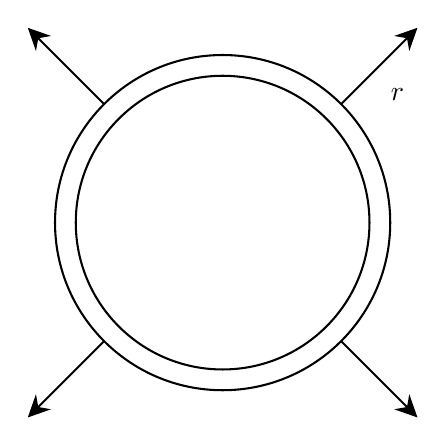
\begin{tikzpicture}[x=0.75pt,y=0.75pt,yscale=-1,xscale=1]
	%uncomment if require: \path (0,300); %set diagram left start at 0, and has height of 300

	%Shape: Circle [id:dp7647812567427628] 
	\draw   (202,140.75) .. controls (202,96.15) and (238.15,60) .. (282.75,60) .. controls (327.35,60) and (363.5,96.15) .. (363.5,140.75) .. controls (363.5,185.35) and (327.35,221.5) .. (282.75,221.5) .. controls (238.15,221.5) and (202,185.35) .. (202,140.75) -- cycle ;
	%Shape: Circle [id:dp8735148170225524] 
	\draw   (212,140.75) .. controls (212,101.68) and (243.68,70) .. (282.75,70) .. controls (321.82,70) and (353.5,101.68) .. (353.5,140.75) .. controls (353.5,179.82) and (321.82,211.5) .. (282.75,211.5) .. controls (243.68,211.5) and (212,179.82) .. (212,140.75) -- cycle ;
	%Straight Lines [id:da05302453801430729] 
	\draw    (339.85,197.85) -- (374.5,232.5) ;
	\draw [shift={(376.62,234.62)}, rotate = 225] [fill={rgb, 255:red, 0; green, 0; blue, 0 }  ][line width=0.08]  [draw opacity=0] (10.72,-5.15) -- (0,0) -- (10.72,5.15) -- (7.12,0) -- cycle    ;
	%Straight Lines [id:da5595293977987936] 
	\draw    (225.65,197.85) -- (191,232.5) ;
	\draw [shift={(188.88,234.62)}, rotate = 315] [fill={rgb, 255:red, 0; green, 0; blue, 0 }  ][line width=0.08]  [draw opacity=0] (10.72,-5.15) -- (0,0) -- (10.72,5.15) -- (7.12,0) -- cycle    ;
	%Straight Lines [id:da29253742485468104] 
	\draw    (191,49) -- (225.65,83.65) ;
	\draw [shift={(188.88,46.88)}, rotate = 45] [fill={rgb, 255:red, 0; green, 0; blue, 0 }  ][line width=0.08]  [draw opacity=0] (10.72,-5.15) -- (0,0) -- (10.72,5.15) -- (7.12,0) -- cycle    ;
	%Straight Lines [id:da6465499849778398] 
	\draw    (374.5,49) -- (339.85,83.65) ;
	\draw [shift={(376.62,46.88)}, rotate = 135] [fill={rgb, 255:red, 0; green, 0; blue, 0 }  ][line width=0.08]  [draw opacity=0] (10.72,-5.15) -- (0,0) -- (10.72,5.15) -- (7.12,0) -- cycle    ;

	% Text Node
	\draw (367,79) node    {$r$};

	\end{tikzpicture}
\end{figure}
\FloatBarrier

\[
	U_m = \frac{1}{2} \frac{B^2}{\mu_0}\cdot \pi r^2 l = \frac{1}{2} \frac{\mu_0^2 n_s^2 I^2}{\mu_0}\cdot \pi r^2 l = \frac{\mu_0 n_s^2 I^2 \pi r^2 l}{2}
\]

La forza vale allora

\[
	F = \frac{dU_m}{dr} = \frac{\mu_0 n_s^2 I^2 \pi l}{2} \cdot 2r = \frac{\mu_0 n_s^2 I^2}{2} \underbrace{2\pi r\,l}_{\Sigma \text{ laterale}}
\]

Vediamo quindi che sulla superficie laterale del tratto di solenoide lungo $l$ agisce la pressione magnetica:

\[
	p_m = \frac{F}{2\pi r\,l} = \frac{\mu_0 n_s^2 I^2}{2} \frac{\mu_0}{\mu_0} = \frac{B^2}{2\mu_0}= u_m
\]

Nella progettazione meccanica di un solenoide bisogna tener conto della pressione magnetica. Ad esempio, in un solenoide capace di produrre un campo $B=1\,T$ la pressione è circa quattro volte quella atmosferica.

\[
	p_m \sim \frac{1}{2\cdot 4\pi \cdot 10^{-7}} \sim \frac{10^6}{2} Pa
\]

L'induttore deve essere in grado di sostenere un campo di questo valore, che tenderebbe a farlo esplodere

\section{Circuiti in mutua induzione}

L'induzione tra due circuiti diventa fondamentale quando si hanno variazioni di corrente e quindi di flusso concatenato tra un circuito e l'altro o anche quando c'è movimento relativo. Due circuiti per cui il coefficiente di induzione mutua non è nullo si dicono accoppiati. Essi sono caratterizzati completamente dalla loro resistenza, dalla loro induttanza e dall'induttanza mutua.

\begin{figure}[htpb]
	\centering

	\tikzset{every picture/.style={line width=0.75pt}} %set default line width to 0.75pt        

	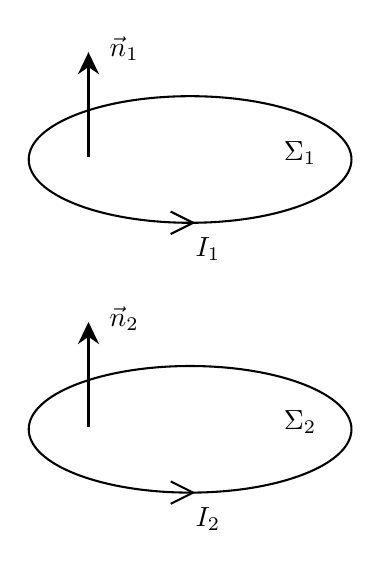
\begin{tikzpicture}[x=0.75pt,y=0.75pt,yscale=-1,xscale=1]
	%uncomment if require: \path (0,300); %set diagram left start at 0, and has height of 300

	%Shape: Ellipse [id:dp022353169953952978] 
	\draw   (192.67,223.17) .. controls (192.67,206.32) and (227.48,192.67) .. (270.42,192.67) .. controls (313.36,192.67) and (348.17,206.32) .. (348.17,223.17) .. controls (348.17,240.01) and (313.36,253.67) .. (270.42,253.67) .. controls (227.48,253.67) and (192.67,240.01) .. (192.67,223.17) -- cycle ;
	\draw   (261.07,248.27) -- (271.87,253.67) -- (261.07,259.07) ;
	%Straight Lines [id:da8413101360434543] 
	\draw    (221.47,221.87) -- (221.47,174.47) ;
	\draw [shift={(221.47,171.47)}, rotate = 450] [fill={rgb, 255:red, 0; green, 0; blue, 0 }  ][line width=0.08]  [draw opacity=0] (10.72,-5.15) -- (0,0) -- (10.72,5.15) -- (7.12,0) -- cycle    ;
	%Shape: Ellipse [id:dp9546111924139196] 
	\draw   (192.67,93.17) .. controls (192.67,76.32) and (227.48,62.67) .. (270.42,62.67) .. controls (313.36,62.67) and (348.17,76.32) .. (348.17,93.17) .. controls (348.17,110.01) and (313.36,123.67) .. (270.42,123.67) .. controls (227.48,123.67) and (192.67,110.01) .. (192.67,93.17) -- cycle ;
	\draw   (261.07,118.27) -- (271.87,123.67) -- (261.07,129.07) ;
	%Straight Lines [id:da19597076868122398] 
	\draw    (221.47,91.87) -- (221.47,44.47) ;
	\draw [shift={(221.47,41.47)}, rotate = 450] [fill={rgb, 255:red, 0; green, 0; blue, 0 }  ][line width=0.08]  [draw opacity=0] (10.72,-5.15) -- (0,0) -- (10.72,5.15) -- (7.12,0) -- cycle    ;

	% Text Node
	\draw (279.07,266.27) node    {$I_{2}$};
	% Text Node
	\draw (323.47,219.87) node    {$\Sigma _{2}$};
	% Text Node
	\draw (238.67,169.87) node    {$\vec{n}_{2}$};
	% Text Node
	\draw (279.07,136.27) node    {$I_{1}$};
	% Text Node
	\draw (323.47,89.87) node    {$\Sigma _{1}$};
	% Text Node
	\draw (238.67,39.87) node    {$\vec{n}_{1}$};

	\end{tikzpicture}
\end{figure}
\FloatBarrier

Il circuito $2$ ($1$) genererà un campo magnetico che provocherà un flusso $\Phi_{21}$ ($\Phi_{12}$) attraverso il circuito $1$ ($2$) dato da:

\[
	\Phi_{21} = \int_{\Sigma_1}  \vec{B}_2 \cdot \vec{n}_1 \, dS = M_{21}\,I_2 \qquad \Phi_{12} = \int_{\Sigma_2}  \vec{B}_1 \cdot \vec{n}_2 \, dS = M_{12}\,I_1
\]

Possiamo immaginare di schematizzare i due circuiti con il simbolismo di sotto

\begin{gather*}
	\Delta V_1 + f_{21} = R_1 I_1 \implies f_{21} = - L_1  \frac{dI_1}{dt} - M \frac{dI_2}{dt} \\
	\Delta V_2 + f_{12} = R_2 I_2 \implies f_{12} = - L_2  \frac{dI_2}{dt} - M \frac{dI_1}{dt}
\end{gather*}

Notiamo che le $f_{21} $ e $f_{12} $ sono date dalla somma della $fem$ di autoinduzione e di quella indotta in un circuito dalla variazione di corrente nell'altro.

\begin{figure}[htpb]
	\centering

	\tikzset{every picture/.style={line width=0.75pt}} %set default line width to 0.75pt        

	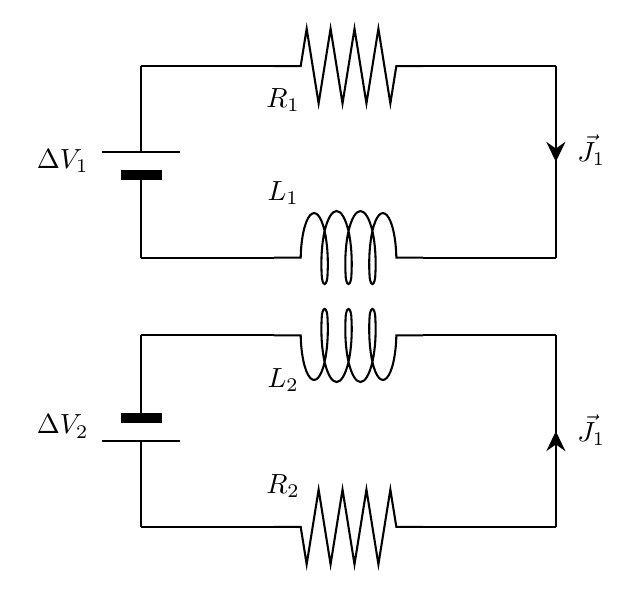
\begin{tikzpicture}[x=0.75pt,y=0.75pt,yscale=-0.9,xscale=0.9]
	%uncomment if require: \path (0,446); %set diagram left start at 0, and has height of 446

	%Straight Lines [id:da5450385787974983] 
	\draw    (229,76) -- (300,76) ;
	%Shape: Resistor [id:dp8836135854518683] 
	\draw   (300,76) -- (314.4,76) -- (317.6,56) -- (324,96) -- (330.4,56) -- (336.8,96) -- (343.2,56) -- (349.6,96) -- (356,56) -- (362.4,96) -- (365.6,76) -- (380,76) ;
	%Shape: Inductor (Air Core) [id:dp5572793678529586] 
	\draw   (300,178.5) -- (314.4,178.5) .. controls (314.61,167.99) and (316.61,159.01) .. (319.43,155.87) .. controls (322.26,152.73) and (325.35,156.07) .. (327.2,164.29) .. controls (328.63,170.7) and (329.21,178.98) .. (328.8,187.03) .. controls (328.8,190.17) and (328.08,192.71) .. (327.2,192.71) .. controls (326.32,192.71) and (325.6,190.17) .. (325.6,187.03) .. controls (325.19,178.98) and (325.77,170.7) .. (327.2,164.29) .. controls (328.86,157.46) and (331.18,153.59) .. (333.6,153.59) .. controls (336.02,153.59) and (338.34,157.46) .. (340,164.29) .. controls (341.43,170.7) and (342.01,178.98) .. (341.6,187.03) .. controls (341.6,190.17) and (340.88,192.71) .. (340,192.71) .. controls (339.12,192.71) and (338.4,190.17) .. (338.4,187.03) .. controls (337.99,178.98) and (338.57,170.7) .. (340,164.29) .. controls (341.66,157.46) and (343.98,153.59) .. (346.4,153.59) .. controls (348.82,153.59) and (351.14,157.46) .. (352.8,164.29) .. controls (354.23,170.7) and (354.81,178.98) .. (354.4,187.03) .. controls (354.4,190.17) and (353.68,192.71) .. (352.8,192.71) .. controls (351.92,192.71) and (351.2,190.17) .. (351.2,187.03) .. controls (350.79,178.98) and (351.37,170.7) .. (352.8,164.29) .. controls (354.65,156.07) and (357.74,152.73) .. (360.57,155.87) .. controls (363.39,159.01) and (365.39,167.99) .. (365.6,178.5) -- (380,178.5) ;
	%Shape: Battery [id:dp46637736818803077] 
	\draw  [fill={rgb, 255:red, 0; green, 0; blue, 0 }  ,fill opacity=1 ] (229,178.5) -- (229,132.38) (208,122.13) -- (250,122.13) (229,122.13) -- (229,76) (218.5,136.48) -- (218.5,132.38) -- (239.5,132.38) -- (239.5,136.48) -- (218.5,136.48) -- cycle ;
	%Straight Lines [id:da5138357380761005] 
	\draw    (380,76) -- (451,76) ;
	%Straight Lines [id:da11798535931656229] 
	\draw    (451,76) -- (451,178.5) ;
	\draw [shift={(451,127.25)}, rotate = 270] [fill={rgb, 255:red, 0; green, 0; blue, 0 }  ][line width=0.08]  [draw opacity=0] (10.72,-5.15) -- (0,0) -- (10.72,5.15) -- (7.12,0) -- cycle    ;
	%Straight Lines [id:da7247473825711936] 
	\draw    (380,178.5) -- (451,178.5) ;
	%Straight Lines [id:da6229977282962058] 
	\draw    (229,178.5) -- (300,178.5) ;
	%Straight Lines [id:da5438168256387526] 
	\draw    (229,322.71) -- (300,322.71) ;
	%Shape: Resistor [id:dp03383264680160458] 
	\draw   (300,322.71) -- (314.4,322.71) -- (317.6,342.71) -- (324,302.71) -- (330.4,342.71) -- (336.8,302.71) -- (343.2,342.71) -- (349.6,302.71) -- (356,342.71) -- (362.4,302.71) -- (365.6,322.71) -- (380,322.71) ;
	%Shape: Inductor (Air Core) [id:dp2169359568934608] 
	\draw   (300,220.21) -- (314.4,220.21) .. controls (314.61,230.72) and (316.61,239.7) .. (319.43,242.85) .. controls (322.26,245.99) and (325.35,242.65) .. (327.2,234.43) .. controls (328.63,228.02) and (329.21,219.73) .. (328.8,211.69) .. controls (328.8,208.55) and (328.08,206) .. (327.2,206) .. controls (326.32,206) and (325.6,208.55) .. (325.6,211.69) .. controls (325.19,219.73) and (325.77,228.02) .. (327.2,234.43) .. controls (328.86,241.26) and (331.18,245.13) .. (333.6,245.13) .. controls (336.02,245.13) and (338.34,241.26) .. (340,234.43) .. controls (341.43,228.02) and (342.01,219.73) .. (341.6,211.69) .. controls (341.6,208.55) and (340.88,206) .. (340,206) .. controls (339.12,206) and (338.4,208.55) .. (338.4,211.69) .. controls (337.99,219.73) and (338.57,228.02) .. (340,234.43) .. controls (341.66,241.26) and (343.98,245.13) .. (346.4,245.13) .. controls (348.82,245.13) and (351.14,241.26) .. (352.8,234.43) .. controls (354.23,228.02) and (354.81,219.73) .. (354.4,211.69) .. controls (354.4,208.55) and (353.68,206) .. (352.8,206) .. controls (351.92,206) and (351.2,208.55) .. (351.2,211.69) .. controls (350.79,219.73) and (351.37,228.02) .. (352.8,234.43) .. controls (354.65,242.65) and (357.74,245.99) .. (360.57,242.85) .. controls (363.39,239.7) and (365.39,230.72) .. (365.6,220.21) -- (380,220.21) ;
	%Shape: Battery [id:dp7599691141751248] 
	\draw  [fill={rgb, 255:red, 0; green, 0; blue, 0 }  ,fill opacity=1 ] (229,220.21) -- (229,266.34) (208,276.59) -- (250,276.59) (229,276.59) -- (229,322.71) (218.5,262.24) -- (218.5,266.34) -- (239.5,266.34) -- (239.5,262.24) -- (218.5,262.24) -- cycle ;
	%Straight Lines [id:da47980589411006647] 
	\draw    (380,322.71) -- (451,322.71) ;
	%Straight Lines [id:da14423806812067075] 
	\draw    (451,322.71) -- (451,220.21) ;
	\draw [shift={(451,271.46)}, rotate = 450] [fill={rgb, 255:red, 0; green, 0; blue, 0 }  ][line width=0.08]  [draw opacity=0] (10.72,-5.15) -- (0,0) -- (10.72,5.15) -- (7.12,0) -- cycle    ;
	%Straight Lines [id:da2656525495579487] 
	\draw    (380,220.21) -- (451,220.21) ;
	%Straight Lines [id:da07229214274510931] 
	\draw    (229,220.21) -- (300,220.21) ;

	% Text Node
	\draw (305,94) node    {$R_{1}$};
	% Text Node
	\draw (305,144) node    {$L_{1}$};
	% Text Node
	\draw (470,121) node    {$\vec{J}_{1}$};
	% Text Node
	\draw (187,127) node    {$\Delta V_{1}$};
	% Text Node
	\draw (305,244) node    {$L_{2}$};
	% Text Node
	\draw (305,301) node    {$R_{2}$};
	% Text Node
	\draw (470,271) node    {$\vec{J}_{1}$};
	% Text Node
	\draw (187,269) node    {$\Delta V_{2}$};

	\end{tikzpicture}
\end{figure}
\FloatBarrier

Otteniamo quindi il seguente sistema di equazione differenziali accoppiate:

\[
	\Delta V_1 - L_1  \frac{dI_1}{dt} - M \frac{dI_2}{dt} = R_1I_1  \qquad  \Delta V_2 - L_2  \frac{dI_2}{dt} - M \frac{dI_1}{dt} = R_2I_2
\]

Dove il termine di accoppiamento in ciascuna è quello contenente $M$.

\section{Energia magnetica di circuiti accoppiati}

Facciamo un analisi del bilancio energetico del sistema visto nel paragrafo precedente.

\begin{gather*}
	I_1\,dt\,\Delta V_1 = I_1\,dt \left[ R_1I_1+L_1\frac{dI_1}{dt}+M\frac{dI_2}{dt}    \right] \\
	I_2\,dt\,\Delta V_2 = I_2\,dt \left[ R_2I_2+L_2\frac{dI_2}{dt}+M\frac{dI_1}{dt}    \right]
\end{gather*}

Sommando il tutto, dato che siamo interessati all'energia legata al sistema nel complesso si ottiene il lavoro che i due generatori compiono nell'istante di tempo.

\begin{align*}
	\Delta V_1I_1dt + \Delta V_2I_2dt &= (R_1I_1^2 +R_2I_2^2 )dt + \\
	&\quad + (L_1I_1dI_1+L_2I_2dI_2) + \tag*{$d\mathcal{L}_{ai} $}\\
	&\quad + (MI_1dI_2 + MI_2dI_1) \tag*{$d\mathcal{L}_{mi} $}
\end{align*}

L'ultimo termine è il lavoro di mutua induzione. Quello al centro è il lavoro di autoinduzione.

\begin{align*}
	\mathcal{L} = U_m &= \int d\mathcal{L}_{ai} + \int d\mathcal{L}_{mi} \\
	&= \int_0^{I_{1\infty}} L_1I_1dI_1 + \int_0^{I_{2\infty}} L_2I_2dI_2 + \iint_0^{I_{1\infty}I_{2\infty}} M d(I_1I_2) \\		&= \frac{1}{2} L_1I_{1\infty}^2 + \frac{1}{2} L_2I_{2\infty}^2 + MI_{1\infty}I_{2\infty}
\end{align*}

L'ultimo termine è chiamata \textbf{energia di accoppiamento}. L'energia non è solo quella che serve per creare il campo separatamente, ma c'è un termine di interazione che deve essere preso in considerazione.
Per estendere il calcolo dell'energia magnetica ad un sistema di $n$ circuiti accoppiati riscriviamo l'ultima espressione trovata per Um in modo che sia suscettibile di generalizzazione. Posto $L_1=M_{11}$, $L_2=M_{22}$ si ha, per $n$ circuiti:

\begin{align*}
	U_m &= \frac{1}{2} M_{11} I_1^2 + \frac{1}{2} M_{22}I_2^2 + \frac{1}{2} M_{12}I_1I_2 + \frac{1}{2} M_{21}I_2I_1 = \frac{1}{2}  \sum_{k,i=1}^n M_{ik}I_iI_k   \\
	U_m &= \frac{1}{2} L_1I_{1\infty}^2 + \frac{1}{2} M_{21} I_{1\infty}I_{2\infty} + \frac{1}{2} L_2I_{2\infty}^2  + \frac{1}{2}  M_{12}I_{2\infty}I_{1\infty} \\
	&= \frac{I_{1\infty}}{2} \underbrace{(L_1I_{1\infty} +M_{21}I_{2\infty})}_{\Phi_1} +\frac{I_{2\infty}}{2} \underbrace{(L_2I_{2\infty} +M_{12}I_{I\infty})}_{\Phi_2} \\
	&= \frac{1}{2} \sum_{i=1}^n I_i\Phi_i
\end{align*}

Questa espressione contiene tutti i flussi di tutti i campi magnetici che passano attraverso il circuito $i$-esimo.

\section{Corrente di spostamento, legge di Ampere - Maxwell}

In regime stazionario la corrente ha gli stessi valori in tutti i punti di un filo conduttore e quindi, qualunque superficie io scelga, la corrente concatenata è sempre la stessa. Nella legge di Ampere quindi, la superficie $ \Sigma  $ attraverso cui si calcola il flusso della densità di corrente è una qualsiasi superficie avente come contorno la linea che concatena $I$ e lungo cui si calcola la circuitazione di $\vec{B}$. Applicando l'operatore divergenza alla quarta equazione di Maxwell abbiamo constatato che essa è in accordo con la conservazione della carica elettrica solo in regime stazionario. Infatti calcolando la divergenza di entrambi i membri dell'equazione si trova:

\[
	\vec{\nabla} (\vec{\nabla} \times \vec{B}) = 0 = \mu_0 \vec{\nabla} \vec{J}_c \implies \vec{\nabla} \vec{J}_c = 0
\]

Che è appunto la forma differenziale della legge di conservazione della carica elettrica nei processi non dipendenti dal tempo. Ma nel caso generale in cui la densità di carica varia nel tempo, la densità di corrente non ha divergenza nulla. La non validità della legge di Ampere in condizioni non stazionarie si può constatare nel processo di carica di un condensatore.
In regime variabile nel tempo, circolerà una corrente $I(t)$. Sulle armature di questo condensatore si accumula o si scarica della quantità di carica in funzione del tempo. Supponiamo di voler determinare il campo magnetico nella regione all'interno del condensatore. Consideriamo una linea chiusa $\lambda$ e calcoliamo la circuitazione di $\vec{B}$ lungo $\lambda$. Scegliamo due superfici $\Sigma_1$ e $\Sigma_2$ come in figura. Attraverso una superficie chiusa che racchiude le armature abbiamo un flusso netto di carica che è nullo, come se ci fosse continuità nel circuito.

\begin{figure}[htpb]
	\centering

	\tikzset{every picture/.style={line width=0.75pt}} %set default line width to 0.75pt        

	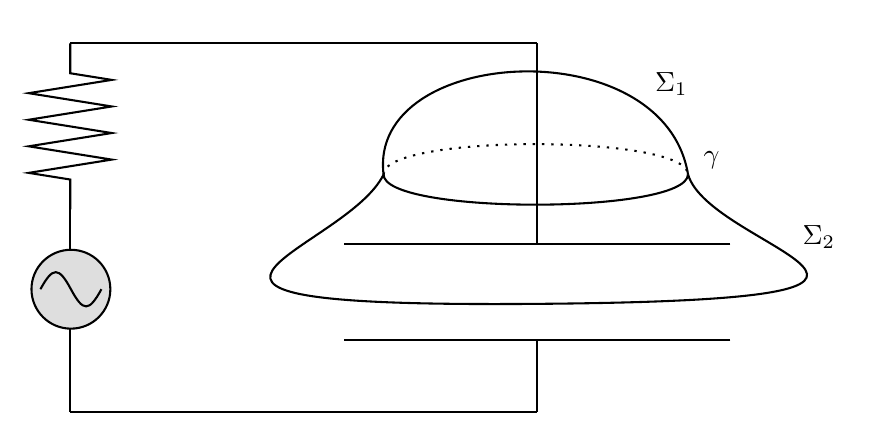
\begin{tikzpicture}[x=0.75pt,y=0.75pt,yscale=-1,xscale=1]
	%uncomment if require: \path (0,300); %set diagram left start at 0, and has height of 300

	%Straight Lines [id:da26715603099101415] 
	\draw    (313,64.5) -- (313,126.67) ;
	%Shape: Contact [id:dp9021730769009411] 
	\draw   (313,126.67) -- (313,161.27) (313,242) -- (313,207.4) (406,161.27) -- (220,161.27) (406,207.4) -- (220,207.4) ;
	%Curve Lines [id:da17311446532911834] 
	\draw    (238.97,127.71) .. controls (231.22,65.58) and (374.04,57.44) .. (385.65,127.63) ;
	%Curve Lines [id:da04270615963409807] 
	\draw    (238.97,127.71) .. controls (229.55,146.77) and (192.04,162.87) .. (185.38,173.94) .. controls (178.72,185.01) and (202.92,191.04) .. (316.92,189.97) .. controls (430.91,188.9) and (450.73,182.47) .. (440.73,171.72) .. controls (430.72,160.98) and (390.91,145.93) .. (385.65,127.63) ;
	%Shape: Resistor [id:dp06847943880021123] 
	\draw   (88,64.5) -- (88,78.9) -- (108,82.1) -- (68,88.5) -- (108,94.9) -- (68,101.3) -- (108,107.7) -- (68,114.1) -- (108,120.5) -- (68,126.9) -- (88,130.1) -- (88,144.5) ;
	%Straight Lines [id:da6677276818736742] 
	\draw    (88,64.5) -- (313,64.5) ;
	%Straight Lines [id:da11229733873192393] 
	\draw    (88,144.5) -- (88,242) ;
	%Straight Lines [id:da9496446795307356] 
	\draw    (88,242) -- (313,242) ;
	%Shape: Circle [id:dp5729624003302884] 
	\draw  [fill={rgb, 255:red, 222; green, 222; blue, 222 }  ,fill opacity=1 ] (69.33,182.95) .. controls (69.33,172.45) and (77.84,163.95) .. (88.33,163.95) .. controls (98.83,163.95) and (107.33,172.45) .. (107.33,182.95) .. controls (107.33,193.44) and (98.83,201.95) .. (88.33,201.95) .. controls (77.84,201.95) and (69.33,193.44) .. (69.33,182.95) -- cycle ;
	%Shape: Sine Wave Form [id:dp12969099670743334] 
	\draw   (73.64,182.95) .. controls (79.62,172.02) and (82.44,171.97) .. (88.33,182.95) .. controls (94.23,193.94) and (96.99,194.01) .. (103.03,182.95) ;

	%Curve Lines [id:da23731231610916503] 
	\draw  [dash pattern={on 0.84pt off 2.51pt}]  (238.97,127.71) .. controls (238.33,108.17) and (385.33,108.17) .. (385.65,127.63) ;
	%Curve Lines [id:da42849339813073684] 
	\draw    (238.97,127.55) .. controls (238.33,147.09) and (385.33,147.09) .. (385.65,127.63) ;

	% Text Node
	\draw (397,120.67) node    {$\gamma $};
	% Text Node
	\draw (377.67,84) node    {$\Sigma _{1}$};
	% Text Node
	\draw (448.67,158) node    {$\Sigma _{2}$};

	\end{tikzpicture}
\end{figure}
\FloatBarrier

Se consideriamo una superficie chiusa che racchiude una sola armatura il flusso di $\vec{J}$ non è nullo perché c'è una carica entrante o uscente, ma nello spazio tra le armature del condensatore non c'è nessun passaggio di carica. Il problema non è ben posto: il concetto di concatenazione funziona in regime stazionario. In tal caso non ci sarebbero correnti concatenate alle due superfici perché la carica sul condensatore è pari a zero. Maxwell propose di estendere il significato della densità di corrente. Il principio di conservazione della carica si può esprimere con il principio di continuità della corrente:

\[
	\left. \begin{array}{r}
	 	\vec{\nabla} \cdot \vec{J}_c = -\frac{\partial \rho_{\text{lib}}}{\partial t} \\
		\vec{\nabla} \cdot \vec{D} = \rho_{\text{lib}}
	\end{array} \right\} \implies \vec{\nabla} \cdot \vec{J}_c = - \frac{\partial}{\partial t} [\vec{\nabla} \cdot \vec{D} ]
\]

Quindi

\[
	\vec{\nabla} \cdot \left[ \vec{J}_c + \underbrace{\frac{\partial \vec{D}}{\partial t}}_{\vec{J}_s} \right] = 0
\]

La quantità $ \vec{J}_s = \frac{\partial \vec{D}}{\partial t} $ viene chiamata \textbf{densità di corrente di spostamento}. Dentro la quadra abbiamo la somma di due densità di corrente, che chiamiamo $\vec{J}_{\text{tot}}$, densità di corrente totale generalizzata $ \vec{J}_{\text{tot}} = \vec{J}_c + \vec{J}_s $. Abbiamo trovato una nuova densità di corrente che è sempre solenoidale in ogni regime. Nel circuito $RC$, sulla superficie $ \Sigma_2  $ è nulla la densità di corrente di conduzione, ma è diverso da zero il campo elettrico generato dalle cariche che stanno sulle armature. D'altra parte su $ \Sigma_1  $ possiamo pensare nullo $\vec{E}$

\[
	\vec{\nabla} \cdot \vec{J}_{\text{tot}} = 0 \implies \int_{\Sigma}\vec{J}_{\text{tot}}\cdot \vec{n} \,dS = 0
\]

Che possiamo pensare come somma dei flussi

\begin{equation*}
	\begin{aligned}
		\int_{\Sigma}\vec{J}_{\text{tot}}\cdot \vec{n} \,dS &= 0 \\
		\underbrace{\int_{\Sigma_1}\vec{J}_{\text{tot}}\cdot (-\vec{n}_1)  \,dS}_{-I_{\text{tot}1}} + \underbrace{\int_{\Sigma_2}\vec{J}_{\text{tot}}\cdot \vec{n}_2 \,dS}_{I_{\text{tot}2}} &= 0 \implies \boxed{I_{\text{tot}1}=I_{\text{tot}2}}
	\end{aligned}
\end{equation*}
$\vec{J}_{\text{tot}} $ ha lo stesso valore in tutto il circuito: esso coincide con la corrente di conduzione nei cavi di collegamento e con la corrente di spostamento all'interno del condensatore.

Nei conduttori di solito $ \vec{J}_s  $ è trascurabile rispetto a $ \vec{J}_c $.

\begin{equation*}
	\begin{aligned}
		I_{\text{tot}1} &= \int_{\Sigma_1} \vec{J}_{\text{tot}} \cdot \vec{n}_1 \,dS = \int_{\Sigma_1} [\vec{J}_c+\vec{J}_s ] \cdot \vec{n}_1 \,dS \simeq \int_{\Sigma_1} \vec{J}_c \cdot \vec{n}_1 \,dS = I_c \\
		I_{\text{tot}2} &= \int_{\Sigma_2} \vec{J}_{\text{tot}} \cdot \vec{n}_2 \,dS = \int_{\Sigma_2} [\vec{J}_c+\vec{J}_s ] \cdot \vec{n}_2 \,dS \simeq \int_{\Sigma_2} \vec{J}_s \cdot \vec{n}_1 \,dS = I_s \\
	\end{aligned}
\end{equation*}

Inoltre

\[
	I_s = \int_{\Sigma_2} \vec{J}_s \cdot \vec{n}_1 \,dS = \int_{\Sigma_2} \frac{\partial \vec{D}}{\partial t} \cdot \vec{n}_1 \,dS = \frac{\partial}{\partial t} \int_{\Sigma_2} \vec{D} \cdot \vec{n}_1 = \frac{\partial \Phi_{\Sigma_2} \vec{D}}{\partial t} \,dS
\]

Abbiamo quindi un nuovo modo per definire in modo corretto il problema di concatenazione grazie a questa nuova densità di corrente generalizzata. Possiamo finalmente calcolare la circuitazione del campo magnetico lungo $ \lambda $:

\[
	\boxed{\oint_{\gamma} \vec{B} \cdot d\vec{l} = \mu_0 \,I_{\text{tot}}}
\]

Questo risultato è chiamato legge di Ampere-Maxwell: essa attribuisce gli stessi effetti magnetici di una corrente di conduzione alle variazioni temporali del campo elettrico. Il termine corrente di spostamento non deve trarre in inganno: alla densità non è collegato nessun moto di carica. La legge ci porta ad un risultato simile alla legge di Faraday. Nel primo caso si parla della circuitazione di $\vec{B}$, nel secondo caso di quella di $\vec{E}$.

\begin{equation*}
	\begin{aligned}
		\oint_{\gamma} \vec{B} \cdot d\vec{l} &= \mu_0 I_{\text{tot}} \\
		\int_{\Sigma} \text{rot}\vec{B} \cdot \vec{n} \, dS &= \mu_0 \int_{\Sigma}\vec{J}_{\text{tot}}\cdot \vec{n} \, dS \\
		\int_{\Sigma} \text{rot}\vec{B} \cdot \vec{n} \, dS &= \int_{\Sigma}\mu_0 \left[ \vec{J}_c + \frac{\partial \vec{D}}{\partial t} \right] \cdot \vec{n} \, dS
	\end{aligned}
\end{equation*}

Queste due espressioni sono sempre uguali qualunque sia la scelta di $\Sigma$ perché l'uguaglianza deriva dal teorema di Stokes e da una legge generalizzata da Maxwell. Gli integrali sono calcolati sulla stessa superficie, quindi devono essere uguali

\[
	\boxed{\text{rot}\vec{B} = \mu_0 \left(\vec{J}_c + \frac{\partial \vec{D}}{\partial t} \right)}
\]

Potremmo trovarci in una situazione più ampia in cui oltre alle correnti di conduzione può esserci anche un mezzo magnetizzato. Le correnti di magnetizzazione danno un ulteriore contributo al campo e non alterano la solenoidalità di $\vec{J}_{\text{tot}} $

\begin{equation*}
	\begin{aligned}
		\text{rot}\vec{B} &= \mu_0 \left[ \vec{J}_c+\frac{\partial \vec{D}}{\partial t} + \vec{J}_m \right] \\
		\frac{\text{rot}\vec{B}}{\mu_0} &= \left[ \vec{J}_c+\frac{\partial \vec{D}}{\partial t} + \text{rot}\vec{M}  \right] \\
		\text{rot} \left[ \frac{\vec{B}}{\mu_0} - \vec{M}  \right] &= \vec{J}_c + \frac{\partial \vec{D}}{\partial t} \\
	\end{aligned}
\end{equation*}

\[
	\boxed{\text{rot}\vec{H} = \vec{J}_c + \frac{\partial \vec{D}}{\partial t}}
\]
\textbf{Riassunto Equazioni di Maxwell.}

\begin{align}
	\text{div}\vec{D} &= \rho_{\text{lib}} (t) \\
	\text{rot}\vec{E} &= -\frac{\partial \vec{B}}{\partial t} \\
	\text{div}\vec{B} &= 0 \\
	\text{rot}\vec{H} &= \vec{J}_c + \frac{\partial \vec{D}}{\partial t}
\end{align}

A queste bisogna aggiungere le relazioni esplicite tra $ \vec{E}  $ e $ \vec{D}  $ e tra $\vec{B}$ e $ \vec{H}  $. Nei mezzi isotropi e omogeni si ha $ \vec{D} = \varepsilon_0 \varepsilon_r \vec{E}  $. Nei materiali diamagnetici e paramagnetici si ha $ \vec{B} = \mu_0 \mu_r \vec{H} $

\[
	\text{rot}\vec{B} = \mu_0 \left[ \vec{J}_c + \vec{J}_m + \varepsilon_0 \frac{\partial \vec{E}}{\partial t} + \frac{\partial \vec{P}}{\partial t} \right]
\]

Possiamo interpretare la derivata di $\vec{P}$ rispetto al tempo come qualcosa di legato all'oscillazione di dipoli causati da campi magnetici variabili nel tempo. Una situazione particolarmente significativa si ha nello spazio vuoto privo di correnti e di cariche. In tal caso si ha

\[
	\text{rot}\vec{E} = \frac{\partial \vec{B}}{\partial t} \qquad \text{rot}\vec{B} = \mu_0 \varepsilon_0 \frac{\partial \vec{E}}{\partial t}
\]

Ogni campo vettoriale può essere scomposto su tre assi coordinati. In tutto abbiamo sei componenti scalari, sei incognite. Le equazioni a disposizione però sono in numero maggiore:

\begin{itemize}
	\item Le due equazioni sui rotori sono vettoriali
	\item Le equazioni sulle divergenze sono di per sé scalari
\end{itemize}

Abbiamo otto equazioni scalari. Il sistema delle equazioni di Maxwell appare sovradimensionato. \emph{In effetti si può notare che le equazioni che contengono veramente tutte le informazioni sono solo le due equazioni sui rotori}. Le altre due equazioni sono già in accordo con esse. Se uno applica a rotore di $\vec{E}$ o di $\vec{B}$ la divergenza da entrambe le parti si ritrovano le altre equazioni.
\emph{Le due equazioni sulle divergenze sono già in accordo con le altre due. Esse sono qualcosa in più e ci dicono qualcosa sulla struttura dei due campi.} Avremo bisogno di loro per capire come sono fatti i campi studiando la propagazione delle onde elettromagnetiche.
Dalle due equazioni notiamo che se consideriamo il caso nel vuoto, un campo magnetico variabile nel tempo genera un campo elettrico. Ma vale anche il caso contrario. I due aspetti sono sempre assieme, ecco perché si parla di campo elettromagnetico. La caratteristica si può vedere anche quando parliamo di campi in regime stazionario.

\textbf{Esempi.}
Consideriamo una regione in cui è presente un campo magnetico $\vec{B}$ uniforme e costante nel tempo. Poniamo che in questa regione dello spazio l'osservatore veda transitare un carica $q$ con una certa velocità $v$. In questo istante non ci sono campi elettrici. Sulla carica agirà la forza di Lorentz pari a:

\[
	\vec{F} = q\,\vec{v} \times \vec{B}
\]

Supponiamo che da queste parti stia transitando un secondo osservatore che si muove per puro caso con la stessa velocità $v$ della particella. L'osservatore $O'$ vede la particella ferma rispetto a sé.

\[
	\vec{v'}=0
\]

Tuttavia nella meccanica classica quando due osservatori sono su un sistema di riferimento inerziale, misurano le stesse forze. La forza misurata da $O'$ non può essere una forza di Lorentz perché la carica è in quiete. L'osservatore $O$ vedrebbe carica doppia se raddoppiassimo la carica, quindi tale forza deve essere proporzionale alla carica. L'unica spiegazione deve essere che sulla carica agisce un campo elettrico $\vec{E}'$ pari a:

\[
	\vec{E'} = \frac{\vec{F'}}{q} = \frac{\vec{F}}{q} = \vec{v} \times \vec{B}
\]
\emph{Campi elettrici e magnetici non sono invarianti passando da un sistema di riferimento all'altro}. Ci si aspettava che siccome le forze non cambiano, nemmeno i due campi sarebbero dovuti cambiare.

Immaginiamo il seguente sistema. Supponiamo che ci sia un filo uniformemente carico caratterizzato da una certa densità di carica lineare $\lambda$. Vi è inoltre un osservatore $O'$ che si muove parallelamente al filo, esso ha l'impressione che le cariche si spostino in direzione opposta a sé. Ma se c'è una corrente, per la legge di Biot-Savart c'è un campo magnetico

\begin{align*}
	\vec{E} = \frac{\lambda}{2\pi \varepsilon_0 r} \vec{u}_n \qquad \vec{B'} &= \frac{\mu_0 I'}{2\pi r} \vec{u}_{\varphi} = \frac{\mu_0 \lambda v}{2\pi r} \vec{u}_{\varphi} = \varepsilon_0 \mu_0 \frac{\lambda}{2\pi \varepsilon_0 r} v \vec{u}_{\varphi} \\
	&= \mu_0 \varepsilon_0 E \, v \, \vec{u}_{\varphi} = \frac{E\,v}{c^2}\vec{u}_{\varphi} = \vec{E} \times \frac{\vec{v}}{c^2} \\
	&= - \frac{\vec{v}}{c^2} \times \vec{E}
\end{align*}

\begin{figure}[htpb]
	\centering

	\tikzset{every picture/.style={line width=0.75pt}} %set default line width to 0.75pt        

	\begin{tikzpicture}[x=0.75pt,y=0.75pt,yscale=-1,xscale=1]
	%uncomment if require: \path (0,366); %set diagram left start at 0, and has height of 366

	%Straight Lines [id:da6831299920859881] 
	\draw    (164,226.41) -- (200.38,226.41) ;
	\draw [shift={(203.38,226.41)}, rotate = 180] [fill={rgb, 255:red, 0; green, 0; blue, 0 }  ][line width=0.08]  [draw opacity=0] (10.72,-5.15) -- (0,0) -- (10.72,5.15) -- (7.12,0) -- cycle    ;
	%Straight Lines [id:da5079842846749154] 
	\draw    (164,226.41) -- (164,190.04) ;
	\draw [shift={(164,187.04)}, rotate = 450] [fill={rgb, 255:red, 0; green, 0; blue, 0 }  ][line width=0.08]  [draw opacity=0] (10.72,-5.15) -- (0,0) -- (10.72,5.15) -- (7.12,0) -- cycle    ;
	%Straight Lines [id:da46686264765372854] 
	\draw    (164,226.41) -- (138.28,252.13) ;
	\draw [shift={(136.16,254.25)}, rotate = 315] [fill={rgb, 255:red, 0; green, 0; blue, 0 }  ][line width=0.08]  [draw opacity=0] (10.72,-5.15) -- (0,0) -- (10.72,5.15) -- (7.12,0) -- cycle    ;
	%Straight Lines [id:da35801584179398116] 
	\draw    (129,162) -- (517,162) ;
	%Straight Lines [id:da7987795836241427] 
	\draw    (375,162) -- (498,162) ;
	\draw [shift={(501,162)}, rotate = 180] [fill={rgb, 255:red, 0; green, 0; blue, 0 }  ][line width=0.08]  [draw opacity=0] (10.72,-5.15) -- (0,0) -- (10.72,5.15) -- (7.12,0) -- cycle    ;
	%Straight Lines [id:da4216029542897226] 
	\draw    (394,86.41) -- (430.38,86.41) ;
	\draw [shift={(433.38,86.41)}, rotate = 180] [fill={rgb, 255:red, 0; green, 0; blue, 0 }  ][line width=0.08]  [draw opacity=0] (10.72,-5.15) -- (0,0) -- (10.72,5.15) -- (7.12,0) -- cycle    ;
	%Straight Lines [id:da6488797391063266] 
	\draw    (394,86.41) -- (394,50.04) ;
	\draw [shift={(394,47.04)}, rotate = 450] [fill={rgb, 255:red, 0; green, 0; blue, 0 }  ][line width=0.08]  [draw opacity=0] (10.72,-5.15) -- (0,0) -- (10.72,5.15) -- (7.12,0) -- cycle    ;
	%Straight Lines [id:da3740424598573331] 
	\draw    (394,86.41) -- (368.28,112.13) ;
	\draw [shift={(366.16,114.25)}, rotate = 315] [fill={rgb, 255:red, 0; green, 0; blue, 0 }  ][line width=0.08]  [draw opacity=0] (10.72,-5.15) -- (0,0) -- (10.72,5.15) -- (7.12,0) -- cycle    ;

	% Text Node
	\draw (167.8,235.79) node    {$O$};
	% Text Node
	\draw (143,149) node    {$+$};
	% Text Node
	\draw (163,149) node    {$+$};
	% Text Node
	\draw (183,149) node    {$+$};
	% Text Node
	\draw (203,149) node    {$+$};
	% Text Node
	\draw (223,149) node    {$+$};
	% Text Node
	\draw (243,149) node    {$+$};
	% Text Node
	\draw (263,149) node    {$+$};
	% Text Node
	\draw (283,149) node    {$+$};
	% Text Node
	\draw (303,149) node    {$+$};
	% Text Node
	\draw (323,149) node    {$+$};
	% Text Node
	\draw (343,149) node    {$+$};
	% Text Node
	\draw (363,149) node    {$+$};
	% Text Node
	\draw (383,149) node    {$+$};
	% Text Node
	\draw (403,149) node    {$+$};
	% Text Node
	\draw (423,149) node    {$+$};
	% Text Node
	\draw (443,149) node    {$+$};
	% Text Node
	\draw (463,149) node    {$+$};
	% Text Node
	\draw (483,149) node    {$+$};
	% Text Node
	\draw (127.24,253.01) node    {$x$};
	% Text Node
	\draw (214.09,224.67) node    {$y$};
	% Text Node
	\draw (155.03,181.99) node    {$z$};
	% Text Node
	\draw (499,177.33) node    {$I'$};
	% Text Node
	\draw (117,159.33) node    {$\lambda $};
	% Text Node
	\draw (400.8,97.79) node    {$O'$};
	% Text Node
	\draw (356.24,114.01) node    {$x'$};
	% Text Node
	\draw (444.09,84.67) node    {$y'$};
	% Text Node
	\draw (384.03,41.99) node    {$z'$};

	\end{tikzpicture}
\end{figure}
\FloatBarrier

A seconda del sistema in cui ci troviamo si manifestano i due campi. È l'idea alla base della relatività ristretta di Einstein. Egli riconobbe che i due campi fanno parte dello stesso oggetto. Siccome i due campi vettoriali hanno tre componenti ciascuno, per rappresentarli in un unico oggetto usiamo una matrice, il tensore elettromagnetico. Nello spazio tempo quando passo da un sistema di riferimento inerziale a un altro è come se stessi facendo una rotazione di coordinare spazio-temporali e con un nuovo sistema di coordinate le componenti dei vettori cambiano ma il tensore è lo stesso. Campo elettrico e campo magnetico sono le componenti di questo tensore. Cambiando sistema di riferimento facciamo una rotazione delle coordinate: cambiano la componente elettrica e magnetica. Ecco perché passando da un SI ad un altro compaiono i campi, sono solo due facce di un unica medaglia da vedere nel suo complesso. È interessante il fatto che l'elettromagnetismo ha portato alla crisi della fisica classica con lo sviluppo della teoria della relatività.